\documentclass[twoside]{book}

% Packages required by doxygen
\usepackage{fixltx2e}
\usepackage{calc}
\usepackage{doxygen}
\usepackage[export]{adjustbox} % also loads graphicx
\usepackage{graphicx}
\usepackage[utf8]{inputenc}
\usepackage{makeidx}
\usepackage{multicol}
\usepackage{multirow}
\PassOptionsToPackage{warn}{textcomp}
\usepackage{textcomp}
\usepackage[nointegrals]{wasysym}
\usepackage[table]{xcolor}

% NLS support packages
\usepackage[catalan]{babel}

% Font selection
\usepackage[T1]{fontenc}
\usepackage[scaled=.90]{helvet}
\usepackage{courier}
\usepackage{amssymb}
\usepackage{sectsty}
\renewcommand{\familydefault}{\sfdefault}
\allsectionsfont{%
  \fontseries{bc}\selectfont%
  \color{darkgray}%
}
\renewcommand{\DoxyLabelFont}{%
  \fontseries{bc}\selectfont%
  \color{darkgray}%
}
\newcommand{\+}{\discretionary{\mbox{\scriptsize$\hookleftarrow$}}{}{}}

% Page & text layout
\usepackage{geometry}
\geometry{%
  a4paper,%
  top=2.5cm,%
  bottom=2.5cm,%
  left=2.5cm,%
  right=2.5cm%
}
\tolerance=750
\hfuzz=15pt
\hbadness=750
\setlength{\emergencystretch}{15pt}
\setlength{\parindent}{0cm}
\setlength{\parskip}{3ex plus 2ex minus 2ex}
\makeatletter
\renewcommand{\paragraph}{%
  \@startsection{paragraph}{4}{0ex}{-1.0ex}{1.0ex}{%
    \normalfont\normalsize\bfseries\SS@parafont%
  }%
}
\renewcommand{\subparagraph}{%
  \@startsection{subparagraph}{5}{0ex}{-1.0ex}{1.0ex}{%
    \normalfont\normalsize\bfseries\SS@subparafont%
  }%
}
\makeatother

% Headers & footers
\usepackage{fancyhdr}
\pagestyle{fancyplain}
\fancyhead[LE]{\fancyplain{}{\bfseries\thepage}}
\fancyhead[CE]{\fancyplain{}{}}
\fancyhead[RE]{\fancyplain{}{\bfseries\leftmark}}
\fancyhead[LO]{\fancyplain{}{\bfseries\rightmark}}
\fancyhead[CO]{\fancyplain{}{}}
\fancyhead[RO]{\fancyplain{}{\bfseries\thepage}}
\fancyfoot[LE]{\fancyplain{}{}}
\fancyfoot[CE]{\fancyplain{}{}}
\fancyfoot[RE]{\fancyplain{}{\bfseries\scriptsize Generat per Doxygen }}
\fancyfoot[LO]{\fancyplain{}{\bfseries\scriptsize Generat per Doxygen }}
\fancyfoot[CO]{\fancyplain{}{}}
\fancyfoot[RO]{\fancyplain{}{}}
\renewcommand{\footrulewidth}{0.4pt}
\renewcommand{\chaptermark}[1]{%
  \markboth{#1}{}%
}
\renewcommand{\sectionmark}[1]{%
  \markright{\thesection\ #1}%
}

% Indices & bibliography
\usepackage{natbib}
\usepackage[titles]{tocloft}
\setcounter{tocdepth}{3}
\setcounter{secnumdepth}{5}
\makeindex

% Hyperlinks (required, but should be loaded last)
\usepackage{ifpdf}
\ifpdf
  \usepackage[pdftex,pagebackref=true]{hyperref}
\else
  \usepackage[ps2pdf,pagebackref=true]{hyperref}
\fi
\hypersetup{%
  colorlinks=true,%
  linkcolor=blue,%
  citecolor=blue,%
  unicode%
}

% Custom commands
\newcommand{\clearemptydoublepage}{%
  \newpage{\pagestyle{empty}\cleardoublepage}%
}

\usepackage{caption}
\captionsetup{labelsep=space,justification=centering,font={bf},singlelinecheck=off,skip=4pt,position=top}

%===== C O N T E N T S =====

\begin{document}

% Titlepage & ToC
\hypersetup{pageanchor=false,
             bookmarksnumbered=true,
             pdfencoding=unicode
            }
\pagenumbering{alph}
\begin{titlepage}
\vspace*{7cm}
\begin{center}%
{\Large Pràctica P\+R\+O2 (Primavera 2020) \\[1ex]\large Roc Salvador Andreazini }\\
\vspace*{1cm}
{\large Generat per Doxygen 1.8.13}\\
\end{center}
\end{titlepage}
\clearemptydoublepage
\pagenumbering{roman}
\tableofcontents
\clearemptydoublepage
\pagenumbering{arabic}
\hypersetup{pageanchor=true}

%--- Begin generated contents ---
\chapter{Espècies, clusters i arbres}
\label{index}\hypertarget{index}{}\hypertarget{index_exp}{}\section{Explicació\+:}\label{index_exp}
{\bfseries  Resum\+: } La pràctica consisteix en implementar un programa que ens permeti gestionar un conjunt d\textquotesingle{}espècies, que calculi la distància entre aquestes i així ens permeti crear un arbre filogenètic mitjançant l\textquotesingle{}algorisme W\+P\+G\+MA.\hypertarget{index_op}{}\section{Operacions\+:}\label{index_op}
El programa permet les següents operacions\+:


\begin{DoxyItemize}
\item crea\+\_\+especie\+: afegeix una espècie al conjunt d\textquotesingle{}espècies
\item obtener\+\_\+gen\+: retorna el gen de l\textquotesingle{}espècie que es demana
\item distancia\+: retorna la distància entre les dues espècies indicades
\item elimina\+\_\+especie\+: elimina l\textquotesingle{}espècie indicada del conjunt d\textquotesingle{}espècies
\item existe\+\_\+especie\+: retorna si l\textquotesingle{}espècie està present al conjunt
\item lee\+\_\+cjt\+\_\+especies\+: llegeix un número d\textquotesingle{}espècies donat
\item imprime\+\_\+cjt\+\_\+especies\+: imprimeix el conjunt amb el gen de cada espècie
\item tabla\+\_\+distancias\+: imprimeix les distàncies entre totes les espècies
\item inicializa\+\_\+clusters\+: inicialitza el conjunt de clusters a partir de les espècies actuals
\item ejecuta\+\_\+paso\+\_\+wpgma\+: executa un pas de l\textquotesingle{}algorisme W\+P\+G\+MA al conjunt de clusters
\item imprime\+\_\+arbol\+\_\+filogenetico\+: imprimeix l\textquotesingle{}arbre que formen el conjunt de clusters actual
\item imprime\+\_\+cluster\+: imprimeix el cluster donat
\item fin\+: acaba l\textquotesingle{}execució del programa
\end{DoxyItemize}\hypertarget{index_inf}{}\section{Informació\+:}\label{index_inf}
{\bfseries  Autor\+: } Roc Salvador Andreazini

{\bfseries  Grup\+: } 11

{\bfseries  Quadrimestre primavera 2020 } 
\chapter{Índex de Classes}
\section{Llista de Classes}
Aquestes són les classes, estructures, unions i interfícies acompanyades amb breus descripcions\+:\begin{DoxyCompactList}
\item\contentsline{section}{\hyperlink{class_cjt__clusters}{Cjt\+\_\+clusters} \\*Representa el conjunt de clusters i les operacions que aquests permeten }{\pageref{class_cjt__clusters}}{}
\item\contentsline{section}{\hyperlink{class_cjt__especies}{Cjt\+\_\+especies} \\*Representa el conjunt d\textquotesingle{}espècies i les operacions que permet }{\pageref{class_cjt__especies}}{}
\item\contentsline{section}{\hyperlink{class_especie}{Especie} \\*Representa una espècie amb els seus atributs i les seves operacions }{\pageref{class_especie}}{}
\end{DoxyCompactList}

\chapter{Índex de Fitxers}
\section{Llista dels Fitxers}
Aquesta és la llista de tots els fitxers acompanyats amb breus descripcions\+:\begin{DoxyCompactList}
\item\contentsline{section}{\hyperlink{_cjt__clusters_8cc}{Cjt\+\_\+clusters.\+cc} \\*Implementació de la classe \hyperlink{class_cjt__clusters}{Cjt\+\_\+clusters} }{\pageref{_cjt__clusters_8cc}}{}
\item\contentsline{section}{\hyperlink{_cjt__clusters_8hh}{Cjt\+\_\+clusters.\+hh} \\*Especificació de la classe \hyperlink{class_cjt__clusters}{Cjt\+\_\+clusters} }{\pageref{_cjt__clusters_8hh}}{}
\item\contentsline{section}{\hyperlink{_cjt__especies_8cc}{Cjt\+\_\+especies.\+cc} \\*Implementació de la classe \hyperlink{_cjt__especies_8cc}{Cjt\+\_\+especies.\+cc} }{\pageref{_cjt__especies_8cc}}{}
\item\contentsline{section}{\hyperlink{_cjt__especies_8hh}{Cjt\+\_\+especies.\+hh} \\*Especificació de la classe \hyperlink{class_cjt__especies}{Cjt\+\_\+especies} }{\pageref{_cjt__especies_8hh}}{}
\item\contentsline{section}{\hyperlink{_especie_8cc}{Especie.\+cc} \\*Implementació de la classe \hyperlink{class_especie}{Especie} }{\pageref{_especie_8cc}}{}
\item\contentsline{section}{\hyperlink{_especie_8hh}{Especie.\+hh} \\*Especificació de la classe \hyperlink{class_especie}{Especie} }{\pageref{_especie_8hh}}{}
\item\contentsline{section}{\hyperlink{program_8cc}{program.\+cc} \\*Programa que conté el main que consisteix en donar diferents operacions }{\pageref{program_8cc}}{}
\end{DoxyCompactList}

\chapter{Documentació de les Classes}
\hypertarget{class_cjt__clusters}{}\section{Referència de la Classe Cjt\+\_\+clusters}
\label{class_cjt__clusters}\index{Cjt\+\_\+clusters@{Cjt\+\_\+clusters}}


Representa el conjunt de clusters i les operacions que aquests permeten.  


\subsection*{Mètodes públics}
\begin{DoxyCompactItemize}
\item 
\hyperlink{class_cjt__clusters_a10dd63eab0e8ea5b1ed13e81412d47a9}{Cjt\+\_\+clusters} ()
\begin{DoxyCompactList}\small\item\em Constructora per defecte. \end{DoxyCompactList}\item 
void \hyperlink{class_cjt__clusters_a0675e6339f6a8fad8219518c377fbcf9}{pas\+\_\+wpgma} ()
\begin{DoxyCompactList}\small\item\em Executa un pas de l\textquotesingle{}algorisme W\+P\+G\+MA amb el cjt\+\_\+clusters actual. \end{DoxyCompactList}\item 
void \hyperlink{class_cjt__clusters_a952291f47c4dd2edf62b3c110bee24f2}{imprimeix\+\_\+arbre\+\_\+filogenetic} ()
\begin{DoxyCompactList}\small\item\em Imprimeix l\textquotesingle{}arbre després d\textquotesingle{}executar tot l\textquotesingle{}algorisme W\+P\+G\+MA. \end{DoxyCompactList}\item 
void \hyperlink{class_cjt__clusters_a928bbb5f0ee0756d291ad28e453892bb}{afegir\+\_\+dist\+\_\+cluster} (const string \&id1, const string \&id2, const double \&dist)
\begin{DoxyCompactList}\small\item\em Afegeix una distància amb una altra espècie. \end{DoxyCompactList}\item 
void \hyperlink{class_cjt__clusters_a2a27f4c57c217eeec5e91777dda19c9d}{afegir\+\_\+cluster} (const string \&id)
\begin{DoxyCompactList}\small\item\em Afegeix un nou cluster al cjt de clusters. \end{DoxyCompactList}\item 
void \hyperlink{class_cjt__clusters_a70aca86e77c34ce652d857b16cc2572f}{neteja\+\_\+clusters} ()
\begin{DoxyCompactList}\small\item\em Elimina tots els elements de la classe cjt clusters. \end{DoxyCompactList}\item 
void \hyperlink{class_cjt__clusters_a732366a2fd16153e162fd838d25b5a56}{imprimeix\+\_\+cluster} (const string \&id) const
\begin{DoxyCompactList}\small\item\em Imprimeix el clúster amb l\textquotesingle{}id donat. \end{DoxyCompactList}\item 
void \hyperlink{class_cjt__clusters_a2ee45d5dabc656adf8d7d356239f57c6}{imprimir\+\_\+taula\+\_\+distancies} () const
\begin{DoxyCompactList}\small\item\em Imprimeix les distàncies de tots els clústers. \end{DoxyCompactList}\item 
bool \hyperlink{class_cjt__clusters_af85ce29152ee18987f391a2d27af59b5}{existeix\+\_\+cluster} (const string \&id) const
\begin{DoxyCompactList}\small\item\em Retorna si existeix un clúser amb id dins del cjt\+\_\+clusters. \end{DoxyCompactList}\item 
int \hyperlink{class_cjt__clusters_a6a240452c7964e1d6b7d54df7ee58563}{num\+\_\+clusters} () const
\begin{DoxyCompactList}\small\item\em Retorna el numero de clusters de la taula de distàncies. \end{DoxyCompactList}\item 
\hyperlink{class_cjt__clusters_aba7f00077ce77ba7963ac8084be4a000}{$\sim$\+Cjt\+\_\+clusters} ()
\begin{DoxyCompactList}\small\item\em Desctructora per defecte. \end{DoxyCompactList}\end{DoxyCompactItemize}
\subsection*{Tipus Privats}
\begin{DoxyCompactItemize}
\item 
typedef map$<$ string, double $>$ \hyperlink{class_cjt__clusters_a9138a363184004ad38221f340abfccd5}{dist\+\_\+cluster}
\end{DoxyCompactItemize}
\subsection*{Mètodes Privats}
\begin{DoxyCompactItemize}
\item 
pair$<$ string, string $>$ \hyperlink{class_cjt__clusters_afe0ecfc740e82c1c00f549ef12279673}{calcular\+\_\+min\+\_\+dist} () const
\begin{DoxyCompactList}\small\item\em Retorna els ids dels clusters a menor distància. \end{DoxyCompactList}\item 
void \hyperlink{class_cjt__clusters_a208f3642fdfe3c3ba9eacc659918f6fa}{recalcular\+\_\+distancia\+\_\+wpgma} (const pair$<$ string, string $>$ \&min\+\_\+dist, map$<$ string, double $>$ \&dist\+\_\+nou\+\_\+cluster)
\begin{DoxyCompactList}\small\item\em Actualitza el conjunt de clusters a lpexecutar el pas wpgma. \end{DoxyCompactList}\end{DoxyCompactItemize}
\subsection*{Atributs Privats}
\begin{DoxyCompactItemize}
\item 
map$<$ string, \hyperlink{class_cjt__clusters_a9138a363184004ad38221f340abfccd5}{dist\+\_\+cluster} $>$ \hyperlink{class_cjt__clusters_a8e94e53830e3224d791dcf7dbd0a6082}{distancies}
\begin{DoxyCompactList}\small\item\em Map que conté els clusters i la seva distància amb la resta, no s\textquotesingle{}aguarden distàncies repetides. \end{DoxyCompactList}\item 
map$<$ string, Bin\+Tree$<$ pair$<$ string, double $>$ $>$ $>$ \hyperlink{class_cjt__clusters_aea7d6362517dd16cbd12736a3da50021}{colleccio\+\_\+clusters}
\begin{DoxyCompactList}\small\item\em Arbres dels diferents clusters amb la distància amb els seus fills. \end{DoxyCompactList}\end{DoxyCompactItemize}


\subsection{Descripció Detallada}
Representa el conjunt de clusters i les operacions que aquests permeten. 

Cada cluster està definit per un identificador i les seves distàncies.

Conté totes les operacions necessàries perquè es pugui executar l\textquotesingle{}algorisme W\+P\+G\+MA a partir d\textquotesingle{}un conjunt d\textquotesingle{}espècies i generar l\textquotesingle{}arbre filogenètic.

Les dades de les estructures de dades del conjunt sempre estan ordenades alfabèticament

Les distàncies entre dos clusters només es guarden al cluster amb id més petit. 

Definició a la línia 28 del fitxer Cjt\+\_\+clusters.\+hh.



\subsection{Documentació de les Definicions de Tipus Membre}
\mbox{\Hypertarget{class_cjt__clusters_a9138a363184004ad38221f340abfccd5}\label{class_cjt__clusters_a9138a363184004ad38221f340abfccd5}} 
\index{Cjt\+\_\+clusters@{Cjt\+\_\+clusters}!dist\+\_\+cluster@{dist\+\_\+cluster}}
\index{dist\+\_\+cluster@{dist\+\_\+cluster}!Cjt\+\_\+clusters@{Cjt\+\_\+clusters}}
\subsubsection{\texorpdfstring{dist\+\_\+cluster}{dist\_cluster}}
{\footnotesize\ttfamily typedef map$<$string,double$>$ \hyperlink{class_cjt__clusters_a9138a363184004ad38221f340abfccd5}{Cjt\+\_\+clusters\+::dist\+\_\+cluster}\hspace{0.3cm}{\ttfamily [private]}}



Definició a la línia 30 del fitxer Cjt\+\_\+clusters.\+hh.



\subsection{Documentació del Constructor i el Destructor}
\mbox{\Hypertarget{class_cjt__clusters_a10dd63eab0e8ea5b1ed13e81412d47a9}\label{class_cjt__clusters_a10dd63eab0e8ea5b1ed13e81412d47a9}} 
\index{Cjt\+\_\+clusters@{Cjt\+\_\+clusters}!Cjt\+\_\+clusters@{Cjt\+\_\+clusters}}
\index{Cjt\+\_\+clusters@{Cjt\+\_\+clusters}!Cjt\+\_\+clusters@{Cjt\+\_\+clusters}}
\subsubsection{\texorpdfstring{Cjt\+\_\+clusters()}{Cjt\_clusters()}}
{\footnotesize\ttfamily Cjt\+\_\+clusters\+::\+Cjt\+\_\+clusters (\begin{DoxyParamCaption}{ }\end{DoxyParamCaption})}



Constructora per defecte. 

\begin{DoxyPrecond}{Precondició}
Cert 
\end{DoxyPrecond}
\begin{DoxyPostcond}{Postcondició}
S\textquotesingle{}ha creat un cjt de clusters buit 
\end{DoxyPostcond}


Definició a la línia 19 del fitxer Cjt\+\_\+clusters.\+cc.


\begin{DoxyCode}
19 \{\}
\end{DoxyCode}
\mbox{\Hypertarget{class_cjt__clusters_aba7f00077ce77ba7963ac8084be4a000}\label{class_cjt__clusters_aba7f00077ce77ba7963ac8084be4a000}} 
\index{Cjt\+\_\+clusters@{Cjt\+\_\+clusters}!````~Cjt\+\_\+clusters@{$\sim$\+Cjt\+\_\+clusters}}
\index{````~Cjt\+\_\+clusters@{$\sim$\+Cjt\+\_\+clusters}!Cjt\+\_\+clusters@{Cjt\+\_\+clusters}}
\subsubsection{\texorpdfstring{$\sim$\+Cjt\+\_\+clusters()}{~Cjt\_clusters()}}
{\footnotesize\ttfamily Cjt\+\_\+clusters\+::$\sim$\+Cjt\+\_\+clusters (\begin{DoxyParamCaption}{ }\end{DoxyParamCaption})}



Desctructora per defecte. 

\begin{DoxyPrecond}{Precondició}
Cert 
\end{DoxyPrecond}
\begin{DoxyPostcond}{Postcondició}
S\textquotesingle{}ha eliminat el cjt de clusters 
\end{DoxyPostcond}


Definició a la línia 144 del fitxer Cjt\+\_\+clusters.\+cc.


\begin{DoxyCode}
144 \{\}
\end{DoxyCode}


\subsection{Documentació de les Funcions Membre}
\mbox{\Hypertarget{class_cjt__clusters_afe0ecfc740e82c1c00f549ef12279673}\label{class_cjt__clusters_afe0ecfc740e82c1c00f549ef12279673}} 
\index{Cjt\+\_\+clusters@{Cjt\+\_\+clusters}!calcular\+\_\+min\+\_\+dist@{calcular\+\_\+min\+\_\+dist}}
\index{calcular\+\_\+min\+\_\+dist@{calcular\+\_\+min\+\_\+dist}!Cjt\+\_\+clusters@{Cjt\+\_\+clusters}}
\subsubsection{\texorpdfstring{calcular\+\_\+min\+\_\+dist()}{calcular\_min\_dist()}}
{\footnotesize\ttfamily pair$<$ string, string $>$ Cjt\+\_\+clusters\+::calcular\+\_\+min\+\_\+dist (\begin{DoxyParamCaption}{ }\end{DoxyParamCaption}) const\hspace{0.3cm}{\ttfamily [private]}}



Retorna els ids dels clusters a menor distància. 

\begin{DoxyPrecond}{Precondició}
Número de clusters $>$ 1 
\end{DoxyPrecond}
\begin{DoxyPostcond}{Postcondició}
S\textquotesingle{}ha retornat els strings dels clusters a menor distància ordenats alfabèticament 
\end{DoxyPostcond}


Definició a la línia 32 del fitxer Cjt\+\_\+clusters.\+cc.


\begin{DoxyCode}
32                                                          \{
33     pair<string,string> min\_dist;
34     \textcolor{keywordtype}{double} dist\_min = 101;
35     \textcolor{keywordflow}{for}(map<string,dist\_cluster>::const\_iterator it = \hyperlink{class_cjt__clusters_a8e94e53830e3224d791dcf7dbd0a6082}{distancies}.begin(); it != 
      \hyperlink{class_cjt__clusters_a8e94e53830e3224d791dcf7dbd0a6082}{distancies}.end(); ++it)\{
36         \textcolor{keywordflow}{for}(map<string,double>::const\_iterator it\_1 = it->second.begin(); it\_1 != it->second.end(); ++it\_1)
      \{
37             \textcolor{keywordflow}{if}(it->first != it\_1->first and it\_1->second < dist\_min)\{
38                 min\_dist.first = it->first;
39                 min\_dist.second = it\_1->first;
40                 dist\_min = it\_1->second;
41             \}
42         \}
43     \}
44     \textcolor{keywordflow}{return} min\_dist;
45 \}
\end{DoxyCode}
\mbox{\Hypertarget{class_cjt__clusters_a208f3642fdfe3c3ba9eacc659918f6fa}\label{class_cjt__clusters_a208f3642fdfe3c3ba9eacc659918f6fa}} 
\index{Cjt\+\_\+clusters@{Cjt\+\_\+clusters}!recalcular\+\_\+distancia\+\_\+wpgma@{recalcular\+\_\+distancia\+\_\+wpgma}}
\index{recalcular\+\_\+distancia\+\_\+wpgma@{recalcular\+\_\+distancia\+\_\+wpgma}!Cjt\+\_\+clusters@{Cjt\+\_\+clusters}}
\subsubsection{\texorpdfstring{recalcular\+\_\+distancia\+\_\+wpgma()}{recalcular\_distancia\_wpgma()}}
{\footnotesize\ttfamily void Cjt\+\_\+clusters\+::recalcular\+\_\+distancia\+\_\+wpgma (\begin{DoxyParamCaption}\item[{const pair$<$ string, string $>$ \&}]{min\+\_\+dist,  }\item[{map$<$ string, double $>$ \&}]{dist\+\_\+nou\+\_\+cluster }\end{DoxyParamCaption})\hspace{0.3cm}{\ttfamily [private]}}



Actualitza el conjunt de clusters a lpexecutar el pas wpgma. 

\begin{DoxyPrecond}{Precondició}
Min\+\_\+dist conté dos ids del cjt de clusters ordenats alfabèticament i distancies.\+size() $>$ 1 
\end{DoxyPrecond}
\begin{DoxyPostcond}{Postcondició}
S\textquotesingle{}ha actualitzat la taula de distàncies afegint el nou cluster amb id = id\+\_\+1 + id\+\_\+2 (id1 $<$ id2) afegit les distàncies amb aquest als clusters amb id $<$ id\+\_\+nou\+\_\+cluster i al nou cluster les distàncies amb id $>$ id\+\_\+nou\+\_\+cluster 
\end{DoxyPostcond}


Definició a la línia 47 del fitxer Cjt\+\_\+clusters.\+cc.


\begin{DoxyCode}
47                                                                                                            
                 \{
48     \textcolor{keywordtype}{string} id\_nou\_cluster = min\_dist.first + min\_dist.second;
49     \textcolor{keywordflow}{for}(map<string,dist\_cluster>::iterator it = \hyperlink{class_cjt__clusters_a8e94e53830e3224d791dcf7dbd0a6082}{distancies}.begin(); it != 
      \hyperlink{class_cjt__clusters_a8e94e53830e3224d791dcf7dbd0a6082}{distancies}.end(); ++it)\{
50         \textcolor{keywordtype}{double} dist;
51         \textcolor{keywordtype}{string} id\_actual = it->first;
52         \textcolor{keywordflow}{if}(id\_actual != min\_dist.first and id\_actual != min\_dist.second)\{
53             \textcolor{comment}{//si l'id de l'espècie actual és més petit q l'id del cluster nou més }
54             \textcolor{comment}{//petit vol dir que conté les distàncies amb els clusters que formen el nou cluster}
55             \textcolor{keywordflow}{if}(id\_actual < min\_dist.first)\{ 
56                 dist = (it->second.find(min\_dist.first)->second+it->second.find(min\_dist.second)->second)/2
      ;
57                 it->second.erase(min\_dist.first);
58                 it->second.erase(min\_dist.second);
59                 it->second.insert(make\_pair(id\_nou\_cluster,dist));
60             \}
61             \textcolor{comment}{//si l'id actual és més petit que l'id més gran del nou cluster vol dir que}
62             \textcolor{comment}{//conté les seves distàncies}
63             \textcolor{keywordflow}{else} \textcolor{keywordflow}{if}(id\_actual < min\_dist.second)\{ \textcolor{comment}{// }
64                 dist = it->second.find(min\_dist.second)->second;
65                 it->second.erase(min\_dist.second);
66                 \textcolor{keyword}{auto} aux = dist\_nou\_cluster.find(id\_actual);
67                 dist += aux->second;
68                 dist /= 2;
69                 aux->second = dist;
70             \}
71         \}
72         \textcolor{keywordflow}{else} \textcolor{keywordflow}{if}(id\_actual == min\_dist.first)\{
73             \textcolor{keywordflow}{for}(\textcolor{keyword}{auto} it1 = it->second.begin(); it1 != it->second.end(); ++it1)\{
74                 \textcolor{keywordflow}{if}(it1->first != min\_dist.second)\{
75                     dist\_nou\_cluster.insert(make\_pair(it1->first,it1->second));
76                 \}
77             \}
78         \}
79         \textcolor{keywordflow}{else} \textcolor{keywordflow}{if}(id\_actual == min\_dist.second)\{
80             \textcolor{keywordflow}{for}(\textcolor{keyword}{auto} it1 = it->second.begin(); it1 != it->second.end(); ++it1)\{
81                 \textcolor{keyword}{auto} aux = dist\_nou\_cluster.find(it1->first);
82                 dist = (aux->second + it1->second)/2;
83                 aux->second = dist;
84             \}
85         \}
86     \}
87 \}
\end{DoxyCode}
\mbox{\Hypertarget{class_cjt__clusters_a0675e6339f6a8fad8219518c377fbcf9}\label{class_cjt__clusters_a0675e6339f6a8fad8219518c377fbcf9}} 
\index{Cjt\+\_\+clusters@{Cjt\+\_\+clusters}!pas\+\_\+wpgma@{pas\+\_\+wpgma}}
\index{pas\+\_\+wpgma@{pas\+\_\+wpgma}!Cjt\+\_\+clusters@{Cjt\+\_\+clusters}}
\subsubsection{\texorpdfstring{pas\+\_\+wpgma()}{pas\_wpgma()}}
{\footnotesize\ttfamily void Cjt\+\_\+clusters\+::pas\+\_\+wpgma (\begin{DoxyParamCaption}{ }\end{DoxyParamCaption})}



Executa un pas de l\textquotesingle{}algorisme W\+P\+G\+MA amb el cjt\+\_\+clusters actual. 

\begin{DoxyPrecond}{Precondició}
distancies.\+size() $>$ 1 
\end{DoxyPrecond}
\begin{DoxyPostcond}{Postcondició}
El cjt\+\_\+clusters ha quedat actualitzat amb un nou cluster a la taula distàncies i a l\textquotesingle{}arbre, també s\textquotesingle{}han eliminat els fills del nou cluster de la taula de distàncies i la col·lecció. A la taula de distàncies\+: s\textquotesingle{}han eliminat les distàncies dels fills que hi havia a la taula i s\textquotesingle{}han afegit les distàncies del nou cluster als clusters amb id $<$ id\+\_\+nou\+\_\+cluster i al nou\+\_\+cluster els clusters amb id $>$ id\+\_\+nou\+\_\+cluster. 
\end{DoxyPostcond}


Definició a la línia 89 del fitxer Cjt\+\_\+clusters.\+cc.


\begin{DoxyCode}
89                             \{
90     pair<string,string> min\_dist = \hyperlink{class_cjt__clusters_afe0ecfc740e82c1c00f549ef12279673}{calcular\_min\_dist}();
91 
92     \textcolor{keywordtype}{double} dist\_fills = \hyperlink{class_cjt__clusters_a8e94e53830e3224d791dcf7dbd0a6082}{distancies}.find(min\_dist.first)->second.find(min\_dist.second)->second/2;
93     \textcolor{keywordtype}{string} id\_nou\_cluster = min\_dist.first + min\_dist.second;
94     map<string,double> dist\_nou\_cluster;
95 
96     \hyperlink{class_cjt__clusters_a208f3642fdfe3c3ba9eacc659918f6fa}{recalcular\_distancia\_wpgma}(min\_dist, dist\_nou\_cluster);
97 
98     \hyperlink{class_cjt__clusters_a8e94e53830e3224d791dcf7dbd0a6082}{distancies}.erase(min\_dist.first);
99     \hyperlink{class_cjt__clusters_a8e94e53830e3224d791dcf7dbd0a6082}{distancies}.erase(min\_dist.second);
100     \hyperlink{class_cjt__clusters_a8e94e53830e3224d791dcf7dbd0a6082}{distancies}.insert(make\_pair(id\_nou\_cluster,dist\_nou\_cluster));
101 
102     BinTree<pair<string,double>> nou\_cluster(make\_pair(id\_nou\_cluster,dist\_fills),
103         \hyperlink{class_cjt__clusters_aea7d6362517dd16cbd12736a3da50021}{colleccio\_clusters}.find(min\_dist.first)->second, 
      \hyperlink{class_cjt__clusters_aea7d6362517dd16cbd12736a3da50021}{colleccio\_clusters}.find(min\_dist.second)->second);
104 
105     \hyperlink{class_cjt__clusters_aea7d6362517dd16cbd12736a3da50021}{colleccio\_clusters}.erase(min\_dist.first);
106     \hyperlink{class_cjt__clusters_aea7d6362517dd16cbd12736a3da50021}{colleccio\_clusters}.erase(min\_dist.second);
107     \hyperlink{class_cjt__clusters_aea7d6362517dd16cbd12736a3da50021}{colleccio\_clusters}.insert(make\_pair(id\_nou\_cluster,nou\_cluster));
108 \}
\end{DoxyCode}
\mbox{\Hypertarget{class_cjt__clusters_a952291f47c4dd2edf62b3c110bee24f2}\label{class_cjt__clusters_a952291f47c4dd2edf62b3c110bee24f2}} 
\index{Cjt\+\_\+clusters@{Cjt\+\_\+clusters}!imprimeix\+\_\+arbre\+\_\+filogenetic@{imprimeix\+\_\+arbre\+\_\+filogenetic}}
\index{imprimeix\+\_\+arbre\+\_\+filogenetic@{imprimeix\+\_\+arbre\+\_\+filogenetic}!Cjt\+\_\+clusters@{Cjt\+\_\+clusters}}
\subsubsection{\texorpdfstring{imprimeix\+\_\+arbre\+\_\+filogenetic()}{imprimeix\_arbre\_filogenetic()}}
{\footnotesize\ttfamily void Cjt\+\_\+clusters\+::imprimeix\+\_\+arbre\+\_\+filogenetic (\begin{DoxyParamCaption}{ }\end{DoxyParamCaption})}



Imprimeix l\textquotesingle{}arbre després d\textquotesingle{}executar tot l\textquotesingle{}algorisme W\+P\+G\+MA. 

\begin{DoxyPrecond}{Precondició}
Cert 
\end{DoxyPrecond}
\begin{DoxyPostcond}{Postcondició}
La taula de distàncies i la col·lecció s\textquotesingle{}han quedat amb un sol element (el cluster arrel), l\textquotesingle{}arbre filogenètic ha quedat completat i aquest s\textquotesingle{}ha imprès pel canal estàndard de sortida 
\end{DoxyPostcond}


Definició a la línia 115 del fitxer Cjt\+\_\+clusters.\+cc.


\begin{DoxyCode}
115                                               \{
116     \textcolor{keywordflow}{while}(\hyperlink{class_cjt__clusters_a8e94e53830e3224d791dcf7dbd0a6082}{distancies}.size() > 1)\{
117         \hyperlink{class_cjt__clusters_a0675e6339f6a8fad8219518c377fbcf9}{pas\_wpgma}();
118     \}
119     \hyperlink{_cjt__clusters_8cc_ac7539e7b223cc6042be093b32ac8b016}{imprimir\_arbre}(\hyperlink{class_cjt__clusters_aea7d6362517dd16cbd12736a3da50021}{colleccio\_clusters}.begin()->second);
120 \}
\end{DoxyCode}
\mbox{\Hypertarget{class_cjt__clusters_a928bbb5f0ee0756d291ad28e453892bb}\label{class_cjt__clusters_a928bbb5f0ee0756d291ad28e453892bb}} 
\index{Cjt\+\_\+clusters@{Cjt\+\_\+clusters}!afegir\+\_\+dist\+\_\+cluster@{afegir\+\_\+dist\+\_\+cluster}}
\index{afegir\+\_\+dist\+\_\+cluster@{afegir\+\_\+dist\+\_\+cluster}!Cjt\+\_\+clusters@{Cjt\+\_\+clusters}}
\subsubsection{\texorpdfstring{afegir\+\_\+dist\+\_\+cluster()}{afegir\_dist\_cluster()}}
{\footnotesize\ttfamily void Cjt\+\_\+clusters\+::afegir\+\_\+dist\+\_\+cluster (\begin{DoxyParamCaption}\item[{const string \&}]{id1,  }\item[{const string \&}]{id2,  }\item[{const double \&}]{dist }\end{DoxyParamCaption})}



Afegeix una distància amb una altra espècie. 

\begin{DoxyPrecond}{Precondició}
dist $>$= 0 i id1 != id2 
\end{DoxyPrecond}
\begin{DoxyPostcond}{Postcondició}
S\textquotesingle{}ha afegit (ordenat alfabèticament) dist a la taula de distàncies d\textquotesingle{}id1 la distància amb id2 
\end{DoxyPostcond}


Definició a la línia 21 del fitxer Cjt\+\_\+clusters.\+cc.


\begin{DoxyCode}
21                                                                                               \{
22     \hyperlink{class_cjt__clusters_a8e94e53830e3224d791dcf7dbd0a6082}{distancies}.find(id1)->second.insert(make\_pair(id2,dist));
23 \}
\end{DoxyCode}
\mbox{\Hypertarget{class_cjt__clusters_a2a27f4c57c217eeec5e91777dda19c9d}\label{class_cjt__clusters_a2a27f4c57c217eeec5e91777dda19c9d}} 
\index{Cjt\+\_\+clusters@{Cjt\+\_\+clusters}!afegir\+\_\+cluster@{afegir\+\_\+cluster}}
\index{afegir\+\_\+cluster@{afegir\+\_\+cluster}!Cjt\+\_\+clusters@{Cjt\+\_\+clusters}}
\subsubsection{\texorpdfstring{afegir\+\_\+cluster()}{afegir\_cluster()}}
{\footnotesize\ttfamily void Cjt\+\_\+clusters\+::afegir\+\_\+cluster (\begin{DoxyParamCaption}\item[{const string \&}]{id }\end{DoxyParamCaption})}



Afegeix un nou cluster al cjt de clusters. 

\begin{DoxyPrecond}{Precondició}
id no present al paràmetre implícit 
\end{DoxyPrecond}
\begin{DoxyPostcond}{Postcondició}
S\textquotesingle{}ha afegit (ordenat alfabèticament) el cluster id a l\textquotesingle{}arbre i a la taula de distàncies 
\end{DoxyPostcond}


Definició a la línia 25 del fitxer Cjt\+\_\+clusters.\+cc.


\begin{DoxyCode}
25                                                  \{
26     map<string,double> aux;
27     \hyperlink{class_cjt__clusters_a8e94e53830e3224d791dcf7dbd0a6082}{distancies}.insert(make\_pair(\textcolor{keywordtype}{id},aux));
28     BinTree<pair<string,double>> arbre(make\_pair(\textcolor{keywordtype}{id},-1));
29     \hyperlink{class_cjt__clusters_aea7d6362517dd16cbd12736a3da50021}{colleccio\_clusters}.insert(make\_pair(\textcolor{keywordtype}{id},arbre));
30 \}
\end{DoxyCode}
\mbox{\Hypertarget{class_cjt__clusters_a70aca86e77c34ce652d857b16cc2572f}\label{class_cjt__clusters_a70aca86e77c34ce652d857b16cc2572f}} 
\index{Cjt\+\_\+clusters@{Cjt\+\_\+clusters}!neteja\+\_\+clusters@{neteja\+\_\+clusters}}
\index{neteja\+\_\+clusters@{neteja\+\_\+clusters}!Cjt\+\_\+clusters@{Cjt\+\_\+clusters}}
\subsubsection{\texorpdfstring{neteja\+\_\+clusters()}{neteja\_clusters()}}
{\footnotesize\ttfamily void Cjt\+\_\+clusters\+::neteja\+\_\+clusters (\begin{DoxyParamCaption}{ }\end{DoxyParamCaption})}



Elimina tots els elements de la classe cjt clusters. 

\begin{DoxyPrecond}{Precondició}
Cert 
\end{DoxyPrecond}
\begin{DoxyPostcond}{Postcondició}
El paràmatre implícit ha quedat buit 
\end{DoxyPostcond}


Definició a la línia 110 del fitxer Cjt\+\_\+clusters.\+cc.


\begin{DoxyCode}
110                                   \{
111     \hyperlink{class_cjt__clusters_a8e94e53830e3224d791dcf7dbd0a6082}{distancies}.clear();
112     \hyperlink{class_cjt__clusters_aea7d6362517dd16cbd12736a3da50021}{colleccio\_clusters}.clear();
113 \}
\end{DoxyCode}
\mbox{\Hypertarget{class_cjt__clusters_a732366a2fd16153e162fd838d25b5a56}\label{class_cjt__clusters_a732366a2fd16153e162fd838d25b5a56}} 
\index{Cjt\+\_\+clusters@{Cjt\+\_\+clusters}!imprimeix\+\_\+cluster@{imprimeix\+\_\+cluster}}
\index{imprimeix\+\_\+cluster@{imprimeix\+\_\+cluster}!Cjt\+\_\+clusters@{Cjt\+\_\+clusters}}
\subsubsection{\texorpdfstring{imprimeix\+\_\+cluster()}{imprimeix\_cluster()}}
{\footnotesize\ttfamily void Cjt\+\_\+clusters\+::imprimeix\+\_\+cluster (\begin{DoxyParamCaption}\item[{const string \&}]{id }\end{DoxyParamCaption}) const}



Imprimeix el clúster amb l\textquotesingle{}id donat. 

\begin{DoxyPrecond}{Precondició}
Existeix un clúster amb this-\/$>$id = id 
\end{DoxyPrecond}
\begin{DoxyPostcond}{Postcondició}
S\textquotesingle{}ha imprès l\textquotesingle{}id i estructura arbòrea del clúster pel canal estàndard de sortida 
\end{DoxyPostcond}


Definició a la línia 122 del fitxer Cjt\+\_\+clusters.\+cc.


\begin{DoxyCode}
122                                                           \{
123     \hyperlink{_cjt__clusters_8cc_ac7539e7b223cc6042be093b32ac8b016}{imprimir\_arbre}(\hyperlink{class_cjt__clusters_aea7d6362517dd16cbd12736a3da50021}{colleccio\_clusters}.find(\textcolor{keywordtype}{id})->second);
124 \}
\end{DoxyCode}
\mbox{\Hypertarget{class_cjt__clusters_a2ee45d5dabc656adf8d7d356239f57c6}\label{class_cjt__clusters_a2ee45d5dabc656adf8d7d356239f57c6}} 
\index{Cjt\+\_\+clusters@{Cjt\+\_\+clusters}!imprimir\+\_\+taula\+\_\+distancies@{imprimir\+\_\+taula\+\_\+distancies}}
\index{imprimir\+\_\+taula\+\_\+distancies@{imprimir\+\_\+taula\+\_\+distancies}!Cjt\+\_\+clusters@{Cjt\+\_\+clusters}}
\subsubsection{\texorpdfstring{imprimir\+\_\+taula\+\_\+distancies()}{imprimir\_taula\_distancies()}}
{\footnotesize\ttfamily void Cjt\+\_\+clusters\+::imprimir\+\_\+taula\+\_\+distancies (\begin{DoxyParamCaption}{ }\end{DoxyParamCaption}) const}



Imprimeix les distàncies de tots els clústers. 

\begin{DoxyPrecond}{Precondició}
Cert 
\end{DoxyPrecond}
\begin{DoxyPostcond}{Postcondició}
S\textquotesingle{}han imprès totes les distàncies pel canal estàndard de sortida 
\end{DoxyPostcond}


Definició a la línia 130 del fitxer Cjt\+\_\+clusters.\+cc.


\begin{DoxyCode}
130                                                   \{
131     \textcolor{keywordflow}{for}(map<string,dist\_cluster>::const\_iterator it = \hyperlink{class_cjt__clusters_a8e94e53830e3224d791dcf7dbd0a6082}{distancies}.begin(); it != 
      \hyperlink{class_cjt__clusters_a8e94e53830e3224d791dcf7dbd0a6082}{distancies}.end(); ++it)\{
132         cout << it->first << \textcolor{stringliteral}{":"};
133         \textcolor{keywordflow}{for}(map<string,double>::const\_iterator it\_1 = it->second.begin(); it\_1 != it->second.end(); ++it\_1)
      \{
134             cout << \textcolor{stringliteral}{" "} << it\_1->first << \textcolor{stringliteral}{" ("} << it\_1->second << \textcolor{stringliteral}{")"};
135         \}
136         cout << endl;
137     \}
138 \}
\end{DoxyCode}
\mbox{\Hypertarget{class_cjt__clusters_af85ce29152ee18987f391a2d27af59b5}\label{class_cjt__clusters_af85ce29152ee18987f391a2d27af59b5}} 
\index{Cjt\+\_\+clusters@{Cjt\+\_\+clusters}!existeix\+\_\+cluster@{existeix\+\_\+cluster}}
\index{existeix\+\_\+cluster@{existeix\+\_\+cluster}!Cjt\+\_\+clusters@{Cjt\+\_\+clusters}}
\subsubsection{\texorpdfstring{existeix\+\_\+cluster()}{existeix\_cluster()}}
{\footnotesize\ttfamily bool Cjt\+\_\+clusters\+::existeix\+\_\+cluster (\begin{DoxyParamCaption}\item[{const string \&}]{id }\end{DoxyParamCaption}) const}



Retorna si existeix un clúser amb id dins del cjt\+\_\+clusters. 

\begin{DoxyPrecond}{Precondició}
Cert 
\end{DoxyPrecond}
\begin{DoxyPostcond}{Postcondició}
Retorna cert si i només si el clúster pertany al paràmetre implícit 
\end{DoxyPostcond}


Definició a la línia 126 del fitxer Cjt\+\_\+clusters.\+cc.


\begin{DoxyCode}
126                                                          \{
127     \textcolor{keywordflow}{return} \hyperlink{class_cjt__clusters_aea7d6362517dd16cbd12736a3da50021}{colleccio\_clusters}.find(\textcolor{keywordtype}{id}) != \hyperlink{class_cjt__clusters_aea7d6362517dd16cbd12736a3da50021}{colleccio\_clusters}.end();
128 \}
\end{DoxyCode}
\mbox{\Hypertarget{class_cjt__clusters_a6a240452c7964e1d6b7d54df7ee58563}\label{class_cjt__clusters_a6a240452c7964e1d6b7d54df7ee58563}} 
\index{Cjt\+\_\+clusters@{Cjt\+\_\+clusters}!num\+\_\+clusters@{num\+\_\+clusters}}
\index{num\+\_\+clusters@{num\+\_\+clusters}!Cjt\+\_\+clusters@{Cjt\+\_\+clusters}}
\subsubsection{\texorpdfstring{num\+\_\+clusters()}{num\_clusters()}}
{\footnotesize\ttfamily int Cjt\+\_\+clusters\+::num\+\_\+clusters (\begin{DoxyParamCaption}{ }\end{DoxyParamCaption}) const}



Retorna el numero de clusters de la taula de distàncies. 

\begin{DoxyPrecond}{Precondició}
Cert 
\end{DoxyPrecond}
\begin{DoxyPostcond}{Postcondició}
S\textquotesingle{}ha retornat la mida del paràmetre implícit 
\end{DoxyPostcond}


Definició a la línia 140 del fitxer Cjt\+\_\+clusters.\+cc.


\begin{DoxyCode}
140                                     \{
141     \textcolor{keywordflow}{return} \hyperlink{class_cjt__clusters_a8e94e53830e3224d791dcf7dbd0a6082}{distancies}.size();
142 \}
\end{DoxyCode}


\subsection{Documentació de les Dades Membre}
\mbox{\Hypertarget{class_cjt__clusters_a8e94e53830e3224d791dcf7dbd0a6082}\label{class_cjt__clusters_a8e94e53830e3224d791dcf7dbd0a6082}} 
\index{Cjt\+\_\+clusters@{Cjt\+\_\+clusters}!distancies@{distancies}}
\index{distancies@{distancies}!Cjt\+\_\+clusters@{Cjt\+\_\+clusters}}
\subsubsection{\texorpdfstring{distancies}{distancies}}
{\footnotesize\ttfamily map$<$string,\hyperlink{class_cjt__clusters_a9138a363184004ad38221f340abfccd5}{dist\+\_\+cluster}$>$ Cjt\+\_\+clusters\+::distancies\hspace{0.3cm}{\ttfamily [private]}}



Map que conté els clusters i la seva distància amb la resta, no s\textquotesingle{}aguarden distàncies repetides. 



Definició a la línia 32 del fitxer Cjt\+\_\+clusters.\+hh.

\mbox{\Hypertarget{class_cjt__clusters_aea7d6362517dd16cbd12736a3da50021}\label{class_cjt__clusters_aea7d6362517dd16cbd12736a3da50021}} 
\index{Cjt\+\_\+clusters@{Cjt\+\_\+clusters}!colleccio\+\_\+clusters@{colleccio\+\_\+clusters}}
\index{colleccio\+\_\+clusters@{colleccio\+\_\+clusters}!Cjt\+\_\+clusters@{Cjt\+\_\+clusters}}
\subsubsection{\texorpdfstring{colleccio\+\_\+clusters}{colleccio\_clusters}}
{\footnotesize\ttfamily map$<$string,Bin\+Tree$<$pair$<$string,double$>$ $>$ $>$ Cjt\+\_\+clusters\+::colleccio\+\_\+clusters\hspace{0.3cm}{\ttfamily [private]}}



Arbres dels diferents clusters amb la distància amb els seus fills. 



Definició a la línia 34 del fitxer Cjt\+\_\+clusters.\+hh.



La documentació d\textquotesingle{}aquesta classe es va generar a partir dels següents fitxers\+:\begin{DoxyCompactItemize}
\item 
\hyperlink{_cjt__clusters_8hh}{Cjt\+\_\+clusters.\+hh}\item 
\hyperlink{_cjt__clusters_8cc}{Cjt\+\_\+clusters.\+cc}\end{DoxyCompactItemize}

\hypertarget{class_cjt__especies}{}\section{Referència de la Classe Cjt\+\_\+especies}
\label{class_cjt__especies}\index{Cjt\+\_\+especies@{Cjt\+\_\+especies}}


Representa el conjunt d\textquotesingle{}espècies i les operacions que permet.  


\subsection*{Mètodes públics}
\begin{DoxyCompactItemize}
\item 
\hyperlink{class_cjt__especies_ab297567c73ccd8caefbd8760d90294a1}{Cjt\+\_\+especies} ()
\begin{DoxyCompactList}\small\item\em Constructora per defecte. \end{DoxyCompactList}\item 
void \hyperlink{class_cjt__especies_a542ea997b387b5bac131ba7bcb23aec3}{afegeix\+\_\+especie} (const string \&id, const string \&gen)
\begin{DoxyCompactList}\small\item\em Crea una especie i l\textquotesingle{}afegeix al parametre implicit. \end{DoxyCompactList}\item 
void \hyperlink{class_cjt__especies_a6de3583aff6835d743fc9493c7b38576}{eliminar\+\_\+especie} (const string \&id)
\begin{DoxyCompactList}\small\item\em Elimina una especie del parametre implicit. \end{DoxyCompactList}\item 
void \hyperlink{class_cjt__especies_a12bd759f16126d0e34b06ecf15575456}{llegir\+\_\+cjt\+\_\+especies} ()
\begin{DoxyCompactList}\small\item\em Llegeix n espècies i les afegeix al conjunt. \end{DoxyCompactList}\item 
string \hyperlink{class_cjt__especies_ae6c9a86512b2ed7686741459167b68c9}{obtenir\+\_\+gen} (const string \&id) const
\begin{DoxyCompactList}\small\item\em Retorna el gen de l\textquotesingle{}espècie id. \end{DoxyCompactList}\item 
bool \hyperlink{class_cjt__especies_a7fa2f303eb4e3065d87174a1c3e71942}{existeix\+\_\+especie} (const string \&id) const
\begin{DoxyCompactList}\small\item\em Retorna cert si l\textquotesingle{}espècie és al cjt d\textquotesingle{}espècies. \end{DoxyCompactList}\item 
double \hyperlink{class_cjt__especies_abcea459e5b302c0eda1583b1dc571bff}{consultar\+\_\+distancia} (const string \&id\+\_\+1, const string \&id\+\_\+2) const
\begin{DoxyCompactList}\small\item\em Calcula la distancia entre dues espècies. \end{DoxyCompactList}\item 
void \hyperlink{class_cjt__especies_a568357e9132b16cfe7280e29e6e89cfb}{inicialitza\+\_\+clusters} (\hyperlink{class_cjt__clusters}{Cjt\+\_\+clusters} \&clusters) const
\begin{DoxyCompactList}\small\item\em Inicialitza el cjt de clusters amb el cjt d\textquotesingle{}especies actual. \end{DoxyCompactList}\item 
int \hyperlink{class_cjt__especies_a2539f8918c40587579e1b98be28bdddc}{consultar\+\_\+mida} () const
\begin{DoxyCompactList}\small\item\em Retorna el número d\textquotesingle{}espècies del conjunt. \end{DoxyCompactList}\item 
void \hyperlink{class_cjt__especies_aeb2402fbb6b5cc5eeea31981c51110bc}{imprimir\+\_\+taula\+\_\+distancies} () const
\begin{DoxyCompactList}\small\item\em Imprimeix totes les distàncies del conjunt d\textquotesingle{}espècies. \end{DoxyCompactList}\item 
void \hyperlink{class_cjt__especies_a8bc985ceafb3bb0e5f3c68ba52a36e86}{escriure\+\_\+cjt\+\_\+especies} () const
\begin{DoxyCompactList}\small\item\em Escriu el conjunt d\textquotesingle{}espècies. \end{DoxyCompactList}\item 
\hyperlink{class_cjt__especies_a05182978f6fff11a0fa1cec49514dd5e}{$\sim$\+Cjt\+\_\+especies} ()
\begin{DoxyCompactList}\small\item\em Constructora per defecte. \end{DoxyCompactList}\end{DoxyCompactItemize}
\subsection*{Atributs Privats}
\begin{DoxyCompactItemize}
\item 
map$<$ string, \hyperlink{class_especie}{Especie} $>$ \hyperlink{class_cjt__especies_aa253bc335c8c8176b8ece5c49a15c5f3}{inventari}
\begin{DoxyCompactList}\small\item\em Conjunt d\textquotesingle{}especies, que no guarden distàncies repetides. \end{DoxyCompactList}\end{DoxyCompactItemize}


\subsection{Descripció Detallada}
Representa el conjunt d\textquotesingle{}espècies i les operacions que permet. 

Conté les operacions necessàries per poder gestionar totes les espècies i traspassar tota la informació necessària al conjunt de clusters.

Les dades de la taula de distàncies estan sempre ordenades alfabèticament

Les distàncies només s\textquotesingle{}aguarden a l\textquotesingle{}espècie amb id més petit. 

Definició a la línia 21 del fitxer Cjt\+\_\+especies.\+hh.



\subsection{Documentació del Constructor i el Destructor}
\mbox{\Hypertarget{class_cjt__especies_ab297567c73ccd8caefbd8760d90294a1}\label{class_cjt__especies_ab297567c73ccd8caefbd8760d90294a1}} 
\index{Cjt\+\_\+especies@{Cjt\+\_\+especies}!Cjt\+\_\+especies@{Cjt\+\_\+especies}}
\index{Cjt\+\_\+especies@{Cjt\+\_\+especies}!Cjt\+\_\+especies@{Cjt\+\_\+especies}}
\subsubsection{\texorpdfstring{Cjt\+\_\+especies()}{Cjt\_especies()}}
{\footnotesize\ttfamily Cjt\+\_\+especies\+::\+Cjt\+\_\+especies (\begin{DoxyParamCaption}{ }\end{DoxyParamCaption})}



Constructora per defecte. 

\begin{DoxyPrecond}{Precondició}
Cert 
\end{DoxyPrecond}
\begin{DoxyPostcond}{Postcondició}
S\textquotesingle{}ha creat un cjt d\textquotesingle{}espècies buit 
\end{DoxyPostcond}


Definició a la línia 6 del fitxer Cjt\+\_\+especies.\+cc.


\begin{DoxyCode}
6 \{\}
\end{DoxyCode}
\mbox{\Hypertarget{class_cjt__especies_a05182978f6fff11a0fa1cec49514dd5e}\label{class_cjt__especies_a05182978f6fff11a0fa1cec49514dd5e}} 
\index{Cjt\+\_\+especies@{Cjt\+\_\+especies}!````~Cjt\+\_\+especies@{$\sim$\+Cjt\+\_\+especies}}
\index{````~Cjt\+\_\+especies@{$\sim$\+Cjt\+\_\+especies}!Cjt\+\_\+especies@{Cjt\+\_\+especies}}
\subsubsection{\texorpdfstring{$\sim$\+Cjt\+\_\+especies()}{~Cjt\_especies()}}
{\footnotesize\ttfamily Cjt\+\_\+especies\+::$\sim$\+Cjt\+\_\+especies (\begin{DoxyParamCaption}{ }\end{DoxyParamCaption})}



Constructora per defecte. 

\begin{DoxyPrecond}{Precondició}
Cert 
\end{DoxyPrecond}
\begin{DoxyPostcond}{Postcondició}
S\textquotesingle{}ha eliminat el cjt d\textquotesingle{}espècies 
\end{DoxyPostcond}


Definició a la línia 97 del fitxer Cjt\+\_\+especies.\+cc.


\begin{DoxyCode}
97 \{\}
\end{DoxyCode}


\subsection{Documentació de les Funcions Membre}
\mbox{\Hypertarget{class_cjt__especies_a542ea997b387b5bac131ba7bcb23aec3}\label{class_cjt__especies_a542ea997b387b5bac131ba7bcb23aec3}} 
\index{Cjt\+\_\+especies@{Cjt\+\_\+especies}!afegeix\+\_\+especie@{afegeix\+\_\+especie}}
\index{afegeix\+\_\+especie@{afegeix\+\_\+especie}!Cjt\+\_\+especies@{Cjt\+\_\+especies}}
\subsubsection{\texorpdfstring{afegeix\+\_\+especie()}{afegeix\_especie()}}
{\footnotesize\ttfamily void Cjt\+\_\+especies\+::afegeix\+\_\+especie (\begin{DoxyParamCaption}\item[{const string \&}]{id,  }\item[{const string \&}]{gen }\end{DoxyParamCaption})}



Crea una especie i l\textquotesingle{}afegeix al parametre implicit. 

\begin{DoxyPrecond}{Precondició}
La nova espècie id no està al paràmetre implícit 
\end{DoxyPrecond}
\begin{DoxyPostcond}{Postcondició}
La nova especie s\textquotesingle{}ha afegit (ordenat alfabèticament) al parametre implicit, s\textquotesingle{}han afegit a les espècies amb identificador $<$ id la distància amb espeècie id i a espècie id s\textquotesingle{}han afegit les distàncies amb espècies amb identificador $>$ id 
\end{DoxyPostcond}


Definició a la línia 8 del fitxer Cjt\+\_\+especies.\+cc.


\begin{DoxyCode}
8                                                                      \{
9     \hyperlink{class_especie}{Especie} esp(gen);
10     \textcolor{keyword}{auto} afegit = \hyperlink{class_cjt__especies_aa253bc335c8c8176b8ece5c49a15c5f3}{inventari}.insert(make\_pair(\textcolor{keywordtype}{id},esp));
11     \textcolor{keywordflow}{for}(map<string,Especie>::iterator it = \hyperlink{class_cjt__especies_aa253bc335c8c8176b8ece5c49a15c5f3}{inventari}.begin(); it != 
      \hyperlink{class_cjt__especies_aa253bc335c8c8176b8ece5c49a15c5f3}{inventari}.end(); ++it)\{
12         \textcolor{keywordflow}{if}(\textcolor{keywordtype}{id} != it->first)\{
13             \textcolor{keywordflow}{if}(id < it->first) afegit.first->second.distancia(it->second,it->first);
14             \textcolor{keywordflow}{else} it->second.distancia(esp,\textcolor{keywordtype}{id});
15         \}
16     \}
17 \}
\end{DoxyCode}
\mbox{\Hypertarget{class_cjt__especies_a6de3583aff6835d743fc9493c7b38576}\label{class_cjt__especies_a6de3583aff6835d743fc9493c7b38576}} 
\index{Cjt\+\_\+especies@{Cjt\+\_\+especies}!eliminar\+\_\+especie@{eliminar\+\_\+especie}}
\index{eliminar\+\_\+especie@{eliminar\+\_\+especie}!Cjt\+\_\+especies@{Cjt\+\_\+especies}}
\subsubsection{\texorpdfstring{eliminar\+\_\+especie()}{eliminar\_especie()}}
{\footnotesize\ttfamily void Cjt\+\_\+especies\+::eliminar\+\_\+especie (\begin{DoxyParamCaption}\item[{const string \&}]{id }\end{DoxyParamCaption})}



Elimina una especie del parametre implicit. 

\begin{DoxyPrecond}{Precondició}
L\textquotesingle{}especie id pertany al parametre implicit 
\end{DoxyPrecond}
\begin{DoxyPostcond}{Postcondició}
L\textquotesingle{}especie id s\textquotesingle{}ha eliminat del parametre implicit i s\textquotesingle{}han eliminat les distàncies amb espècie id de les espècies amb identificador $<$ id 
\end{DoxyPostcond}


Definició a la línia 59 del fitxer Cjt\+\_\+especies.\+cc.


\begin{DoxyCode}
59                                                    \{
60     \hyperlink{class_cjt__especies_aa253bc335c8c8176b8ece5c49a15c5f3}{inventari}.erase(\textcolor{keywordtype}{id});
61     map<string,Especie>::iterator it = \hyperlink{class_cjt__especies_aa253bc335c8c8176b8ece5c49a15c5f3}{inventari}.begin();
62     \textcolor{keywordflow}{while}(it != \hyperlink{class_cjt__especies_aa253bc335c8c8176b8ece5c49a15c5f3}{inventari}.end() and it->first < id)\{
63         it->second.eliminar\_esp\_dist(\textcolor{keywordtype}{id});
64         ++it;
65     \}
66 \}
\end{DoxyCode}
\mbox{\Hypertarget{class_cjt__especies_a12bd759f16126d0e34b06ecf15575456}\label{class_cjt__especies_a12bd759f16126d0e34b06ecf15575456}} 
\index{Cjt\+\_\+especies@{Cjt\+\_\+especies}!llegir\+\_\+cjt\+\_\+especies@{llegir\+\_\+cjt\+\_\+especies}}
\index{llegir\+\_\+cjt\+\_\+especies@{llegir\+\_\+cjt\+\_\+especies}!Cjt\+\_\+especies@{Cjt\+\_\+especies}}
\subsubsection{\texorpdfstring{llegir\+\_\+cjt\+\_\+especies()}{llegir\_cjt\_especies()}}
{\footnotesize\ttfamily void Cjt\+\_\+especies\+::llegir\+\_\+cjt\+\_\+especies (\begin{DoxyParamCaption}{ }\end{DoxyParamCaption})}



Llegeix n espècies i les afegeix al conjunt. 

\begin{DoxyPrecond}{Precondició}
Cert 
\end{DoxyPrecond}
\begin{DoxyPostcond}{Postcondició}
S\textquotesingle{}han esborrat les espècies anteriors i s\textquotesingle{}han afegit les espècies llegides al parametre implícit 
\end{DoxyPostcond}


Definició a la línia 38 del fitxer Cjt\+\_\+especies.\+cc.


\begin{DoxyCode}
38                                       \{
39     \hyperlink{class_cjt__especies_aa253bc335c8c8176b8ece5c49a15c5f3}{inventari}.clear();
40     \textcolor{keywordtype}{int} n;
41     cin >> n;
42 
43     \textcolor{keywordtype}{string} id, gen;
44     \textcolor{keywordflow}{for}(\textcolor{keywordtype}{int} i = 0; i < n; ++i)\{
45         cin >> \textcolor{keywordtype}{id} >> gen;
46         \hyperlink{class_especie}{Especie} esp(gen);
47         \hyperlink{class_cjt__especies_aa253bc335c8c8176b8ece5c49a15c5f3}{inventari}.insert(make\_pair(\textcolor{keywordtype}{id},esp));
48     \}
49 
50     \textcolor{keywordflow}{for}(map<string,Especie>::iterator it = \hyperlink{class_cjt__especies_aa253bc335c8c8176b8ece5c49a15c5f3}{inventari}.begin(); it != 
      \hyperlink{class_cjt__especies_aa253bc335c8c8176b8ece5c49a15c5f3}{inventari}.end(); ++it)\{
51         \textcolor{keywordflow}{for}(map<string,Especie>::iterator it\_1 = it; it\_1 != \hyperlink{class_cjt__especies_aa253bc335c8c8176b8ece5c49a15c5f3}{inventari}.end(); ++it\_1)\{
52             \textcolor{keywordflow}{if}(it->first != it\_1->first)\{
53                 it->second.distancia(it\_1->second,it\_1->first);
54             \}
55         \}
56     \}
57 \}
\end{DoxyCode}
\mbox{\Hypertarget{class_cjt__especies_ae6c9a86512b2ed7686741459167b68c9}\label{class_cjt__especies_ae6c9a86512b2ed7686741459167b68c9}} 
\index{Cjt\+\_\+especies@{Cjt\+\_\+especies}!obtenir\+\_\+gen@{obtenir\+\_\+gen}}
\index{obtenir\+\_\+gen@{obtenir\+\_\+gen}!Cjt\+\_\+especies@{Cjt\+\_\+especies}}
\subsubsection{\texorpdfstring{obtenir\+\_\+gen()}{obtenir\_gen()}}
{\footnotesize\ttfamily string Cjt\+\_\+especies\+::obtenir\+\_\+gen (\begin{DoxyParamCaption}\item[{const string \&}]{id }\end{DoxyParamCaption}) const}



Retorna el gen de l\textquotesingle{}espècie id. 

\begin{DoxyPrecond}{Precondició}
L\textquotesingle{}element id pertany al parametre implicit 
\end{DoxyPrecond}
\begin{DoxyPostcond}{Postcondició}
S\textquotesingle{}ha retornat el gen de l\textquotesingle{}identificador 
\end{DoxyPostcond}


Definició a la línia 19 del fitxer Cjt\+\_\+especies.\+cc.


\begin{DoxyCode}
19                                                       \{
20     \textcolor{keywordflow}{return} \hyperlink{class_cjt__especies_aa253bc335c8c8176b8ece5c49a15c5f3}{inventari}.find(\textcolor{keywordtype}{id})->second.consultar\_gen();
21 \}
\end{DoxyCode}
\mbox{\Hypertarget{class_cjt__especies_a7fa2f303eb4e3065d87174a1c3e71942}\label{class_cjt__especies_a7fa2f303eb4e3065d87174a1c3e71942}} 
\index{Cjt\+\_\+especies@{Cjt\+\_\+especies}!existeix\+\_\+especie@{existeix\+\_\+especie}}
\index{existeix\+\_\+especie@{existeix\+\_\+especie}!Cjt\+\_\+especies@{Cjt\+\_\+especies}}
\subsubsection{\texorpdfstring{existeix\+\_\+especie()}{existeix\_especie()}}
{\footnotesize\ttfamily bool Cjt\+\_\+especies\+::existeix\+\_\+especie (\begin{DoxyParamCaption}\item[{const string \&}]{id }\end{DoxyParamCaption}) const}



Retorna cert si l\textquotesingle{}espècie és al cjt d\textquotesingle{}espècies. 

\begin{DoxyPrecond}{Precondició}
Cert 
\end{DoxyPrecond}
\begin{DoxyPostcond}{Postcondició}
S\textquotesingle{}ha retornat cert si l\textquotesingle{}especie pertany al parametre implicit sinó fals 
\end{DoxyPostcond}


Definició a la línia 74 del fitxer Cjt\+\_\+especies.\+cc.


\begin{DoxyCode}
74                                                          \{
75     \textcolor{keywordflow}{return} \hyperlink{class_cjt__especies_aa253bc335c8c8176b8ece5c49a15c5f3}{inventari}.find(\textcolor{keywordtype}{id}) != \hyperlink{class_cjt__especies_aa253bc335c8c8176b8ece5c49a15c5f3}{inventari}.end();
76 \}
\end{DoxyCode}
\mbox{\Hypertarget{class_cjt__especies_abcea459e5b302c0eda1583b1dc571bff}\label{class_cjt__especies_abcea459e5b302c0eda1583b1dc571bff}} 
\index{Cjt\+\_\+especies@{Cjt\+\_\+especies}!consultar\+\_\+distancia@{consultar\+\_\+distancia}}
\index{consultar\+\_\+distancia@{consultar\+\_\+distancia}!Cjt\+\_\+especies@{Cjt\+\_\+especies}}
\subsubsection{\texorpdfstring{consultar\+\_\+distancia()}{consultar\_distancia()}}
{\footnotesize\ttfamily double Cjt\+\_\+especies\+::consultar\+\_\+distancia (\begin{DoxyParamCaption}\item[{const string \&}]{id\+\_\+1,  }\item[{const string \&}]{id\+\_\+2 }\end{DoxyParamCaption}) const}



Calcula la distancia entre dues espècies. 

\begin{DoxyPrecond}{Precondició}
Els paràmetres pertanyen al paràmetre implicit 
\end{DoxyPrecond}
\begin{DoxyPostcond}{Postcondició}
S\textquotesingle{}ha retornat la distancia entre les dues espècies 
\end{DoxyPostcond}


Definició a la línia 68 del fitxer Cjt\+\_\+especies.\+cc.


\begin{DoxyCode}
68                                                                                     \{
69     \textcolor{keywordflow}{if}(id\_1 < id\_2) \textcolor{keywordflow}{return} \hyperlink{class_cjt__especies_aa253bc335c8c8176b8ece5c49a15c5f3}{inventari}.find(id\_1)->second.consultar\_distancia(id\_2);
70     \textcolor{keywordflow}{else} \textcolor{keywordflow}{if}(id\_1 == id\_2) \textcolor{keywordflow}{return} 0;
71     \textcolor{keywordflow}{else} \textcolor{keywordflow}{return} \hyperlink{class_cjt__especies_aa253bc335c8c8176b8ece5c49a15c5f3}{inventari}.find(id\_2)->second.consultar\_distancia(id\_1);
72 \}
\end{DoxyCode}
\mbox{\Hypertarget{class_cjt__especies_a568357e9132b16cfe7280e29e6e89cfb}\label{class_cjt__especies_a568357e9132b16cfe7280e29e6e89cfb}} 
\index{Cjt\+\_\+especies@{Cjt\+\_\+especies}!inicialitza\+\_\+clusters@{inicialitza\+\_\+clusters}}
\index{inicialitza\+\_\+clusters@{inicialitza\+\_\+clusters}!Cjt\+\_\+especies@{Cjt\+\_\+especies}}
\subsubsection{\texorpdfstring{inicialitza\+\_\+clusters()}{inicialitza\_clusters()}}
{\footnotesize\ttfamily void Cjt\+\_\+especies\+::inicialitza\+\_\+clusters (\begin{DoxyParamCaption}\item[{\hyperlink{class_cjt__clusters}{Cjt\+\_\+clusters} \&}]{clusters }\end{DoxyParamCaption}) const}



Inicialitza el cjt de clusters amb el cjt d\textquotesingle{}especies actual. 

\begin{DoxyPrecond}{Precondició}
Cert 
\end{DoxyPrecond}
\begin{DoxyPostcond}{Postcondició}
El paràmetre explícit ha quedat igual que la taula de distàncies de les espècies del paràmetre implícit 
\end{DoxyPostcond}


Definició a la línia 23 del fitxer Cjt\+\_\+especies.\+cc.


\begin{DoxyCode}
23                                                                    \{
24     clusters.\hyperlink{class_cjt__clusters_a70aca86e77c34ce652d857b16cc2572f}{neteja\_clusters}();
25     \textcolor{keywordflow}{for}(map<string,Especie>::const\_iterator it = \hyperlink{class_cjt__especies_aa253bc335c8c8176b8ece5c49a15c5f3}{inventari}.begin(); it != 
      \hyperlink{class_cjt__especies_aa253bc335c8c8176b8ece5c49a15c5f3}{inventari}.end(); ++it)\{
26         \textcolor{keywordflow}{for}(map<string,Especie>::const\_iterator it1 = it; it1 != \hyperlink{class_cjt__especies_aa253bc335c8c8176b8ece5c49a15c5f3}{inventari}.end(); ++it1)\{
27             \textcolor{keywordflow}{if}(it->first != it1->first)\{
28                 \textcolor{keywordtype}{string} id1 = it->first;
29                 \textcolor{keywordtype}{string} id2 = it1->first;
30                 \textcolor{keywordtype}{double} dist = it->second.consultar\_distancia(id2);
31                 clusters.\hyperlink{class_cjt__clusters_a928bbb5f0ee0756d291ad28e453892bb}{afegir\_dist\_cluster}(id1,id2,dist);
32             \}
33             \textcolor{keywordflow}{else} clusters.\hyperlink{class_cjt__clusters_a2a27f4c57c217eeec5e91777dda19c9d}{afegir\_cluster}(it->first);
34         \}
35     \}
36 \}
\end{DoxyCode}
\mbox{\Hypertarget{class_cjt__especies_a2539f8918c40587579e1b98be28bdddc}\label{class_cjt__especies_a2539f8918c40587579e1b98be28bdddc}} 
\index{Cjt\+\_\+especies@{Cjt\+\_\+especies}!consultar\+\_\+mida@{consultar\+\_\+mida}}
\index{consultar\+\_\+mida@{consultar\+\_\+mida}!Cjt\+\_\+especies@{Cjt\+\_\+especies}}
\subsubsection{\texorpdfstring{consultar\+\_\+mida()}{consultar\_mida()}}
{\footnotesize\ttfamily int Cjt\+\_\+especies\+::consultar\+\_\+mida (\begin{DoxyParamCaption}{ }\end{DoxyParamCaption}) const}



Retorna el número d\textquotesingle{}espècies del conjunt. 

\begin{DoxyPrecond}{Precondició}
Cert 
\end{DoxyPrecond}
\begin{DoxyPostcond}{Postcondició}
S\textquotesingle{}ha retornat el valor de la mida del paràmetre implicit 
\end{DoxyPostcond}


Definició a la línia 92 del fitxer Cjt\+\_\+especies.\+cc.


\begin{DoxyCode}
92                                       \{
93     \textcolor{keywordflow}{return} \hyperlink{class_cjt__especies_aa253bc335c8c8176b8ece5c49a15c5f3}{inventari}.size();
94 \}
\end{DoxyCode}
\mbox{\Hypertarget{class_cjt__especies_aeb2402fbb6b5cc5eeea31981c51110bc}\label{class_cjt__especies_aeb2402fbb6b5cc5eeea31981c51110bc}} 
\index{Cjt\+\_\+especies@{Cjt\+\_\+especies}!imprimir\+\_\+taula\+\_\+distancies@{imprimir\+\_\+taula\+\_\+distancies}}
\index{imprimir\+\_\+taula\+\_\+distancies@{imprimir\+\_\+taula\+\_\+distancies}!Cjt\+\_\+especies@{Cjt\+\_\+especies}}
\subsubsection{\texorpdfstring{imprimir\+\_\+taula\+\_\+distancies()}{imprimir\_taula\_distancies()}}
{\footnotesize\ttfamily void Cjt\+\_\+especies\+::imprimir\+\_\+taula\+\_\+distancies (\begin{DoxyParamCaption}{ }\end{DoxyParamCaption}) const}



Imprimeix totes les distàncies del conjunt d\textquotesingle{}espècies. 

\begin{DoxyPrecond}{Precondició}
Cert 
\end{DoxyPrecond}
\begin{DoxyPostcond}{Postcondició}
S\textquotesingle{}han imprès totes les distàncies pel canal estàndard de sortida 
\end{DoxyPostcond}


Definició a la línia 84 del fitxer Cjt\+\_\+especies.\+cc.


\begin{DoxyCode}
84                                                   \{
85     \textcolor{keywordflow}{for}(map<string,Especie>::const\_iterator it = \hyperlink{class_cjt__especies_aa253bc335c8c8176b8ece5c49a15c5f3}{inventari}.begin(); it != 
      \hyperlink{class_cjt__especies_aa253bc335c8c8176b8ece5c49a15c5f3}{inventari}.end(); ++it)\{
86         cout << it->first << \textcolor{stringliteral}{":"};
87         it->second.imprimir\_distancies();
88         cout << endl;
89     \}
90 \}
\end{DoxyCode}
\mbox{\Hypertarget{class_cjt__especies_a8bc985ceafb3bb0e5f3c68ba52a36e86}\label{class_cjt__especies_a8bc985ceafb3bb0e5f3c68ba52a36e86}} 
\index{Cjt\+\_\+especies@{Cjt\+\_\+especies}!escriure\+\_\+cjt\+\_\+especies@{escriure\+\_\+cjt\+\_\+especies}}
\index{escriure\+\_\+cjt\+\_\+especies@{escriure\+\_\+cjt\+\_\+especies}!Cjt\+\_\+especies@{Cjt\+\_\+especies}}
\subsubsection{\texorpdfstring{escriure\+\_\+cjt\+\_\+especies()}{escriure\_cjt\_especies()}}
{\footnotesize\ttfamily void Cjt\+\_\+especies\+::escriure\+\_\+cjt\+\_\+especies (\begin{DoxyParamCaption}{ }\end{DoxyParamCaption}) const}



Escriu el conjunt d\textquotesingle{}espècies. 

\begin{DoxyPrecond}{Precondició}
Cert 
\end{DoxyPrecond}
\begin{DoxyPostcond}{Postcondició}
S\textquotesingle{}han imprès les espècies pel canal estàndard de sortida 
\end{DoxyPostcond}


Definició a la línia 78 del fitxer Cjt\+\_\+especies.\+cc.


\begin{DoxyCode}
78                                               \{
79     \textcolor{keywordflow}{for}(map<string,Especie>::const\_iterator it = \hyperlink{class_cjt__especies_aa253bc335c8c8176b8ece5c49a15c5f3}{inventari}.begin(); it != 
      \hyperlink{class_cjt__especies_aa253bc335c8c8176b8ece5c49a15c5f3}{inventari}.end(); ++it)\{
80         cout << it->first << \textcolor{stringliteral}{" "} << it->second.consultar\_gen() << endl;
81     \}
82 \}
\end{DoxyCode}


\subsection{Documentació de les Dades Membre}
\mbox{\Hypertarget{class_cjt__especies_aa253bc335c8c8176b8ece5c49a15c5f3}\label{class_cjt__especies_aa253bc335c8c8176b8ece5c49a15c5f3}} 
\index{Cjt\+\_\+especies@{Cjt\+\_\+especies}!inventari@{inventari}}
\index{inventari@{inventari}!Cjt\+\_\+especies@{Cjt\+\_\+especies}}
\subsubsection{\texorpdfstring{inventari}{inventari}}
{\footnotesize\ttfamily map$<$string,\hyperlink{class_especie}{Especie}$>$ Cjt\+\_\+especies\+::inventari\hspace{0.3cm}{\ttfamily [private]}}



Conjunt d\textquotesingle{}especies, que no guarden distàncies repetides. 



Definició a la línia 24 del fitxer Cjt\+\_\+especies.\+hh.



La documentació d\textquotesingle{}aquesta classe es va generar a partir dels següents fitxers\+:\begin{DoxyCompactItemize}
\item 
\hyperlink{_cjt__especies_8hh}{Cjt\+\_\+especies.\+hh}\item 
\hyperlink{_cjt__especies_8cc}{Cjt\+\_\+especies.\+cc}\end{DoxyCompactItemize}

\hypertarget{class_especie}{}\section{Referència de la Classe Especie}
\label{class_especie}\index{Especie@{Especie}}


Representa una espècie amb els seus atributs i les seves operacions.  


\subsection*{Mètodes públics}
\begin{DoxyCompactItemize}
\item 
\hyperlink{class_especie_a597cfbcc08d584338ffe2f5105f9e9c1}{Especie} (const string \&\hyperlink{class_especie_ac35bb565f7346cd6317b3a8c849456d1}{gen})
\begin{DoxyCompactList}\small\item\em Creadora. \end{DoxyCompactList}\item 
string \hyperlink{class_especie_a850af2b59a21e2d801c59d76ba5c1a98}{consultar\+\_\+gen} () const
\begin{DoxyCompactList}\small\item\em Consulta el gen de l\textquotesingle{}espècie. \end{DoxyCompactList}\item 
double \hyperlink{class_especie_ae72023f716c9ae50a160f751b0365efe}{consultar\+\_\+distancia} (const string \&id) const
\begin{DoxyCompactList}\small\item\em Consulta la distància amb l\textquotesingle{}espècie id. \end{DoxyCompactList}\item 
void \hyperlink{class_especie_a305c663aa9f2c8b596e940067fdd6177}{imprimir\+\_\+distancies} () const
\begin{DoxyCompactList}\small\item\em Imprimeix les distàncies amb la resta d\textquotesingle{}espècies. \end{DoxyCompactList}\item 
void \hyperlink{class_especie_abe0e84ff19b61d434d501f943a542bc9}{distancia} (const \hyperlink{class_especie}{Especie} \&esp, const string \&id)
\begin{DoxyCompactList}\small\item\em Calcula la distància amb l\textquotesingle{}espècie del paràmetre esplícit i l\textquotesingle{}afegeix al paràmetre implícit. \end{DoxyCompactList}\item 
void \hyperlink{class_especie_a2a63fa33f9297beec7b57a86fe55ce2a}{eliminar\+\_\+esp\+\_\+dist} (const string \&id)
\begin{DoxyCompactList}\small\item\em Elimina la distància amb l\textquotesingle{}espècie id. \end{DoxyCompactList}\item 
\hyperlink{class_especie_abd21378dde6e8348d823c6f87a1c0658}{$\sim$\+Especie} ()
\begin{DoxyCompactList}\small\item\em Destructora per defecte. \end{DoxyCompactList}\end{DoxyCompactItemize}
\subsection*{Mètodes Públics Estàtics}
\begin{DoxyCompactItemize}
\item 
static void \hyperlink{class_especie_a30e274da0f6d1ee4c450702a3f914ecf}{definir\+\_\+k} (const int \&\hyperlink{class_especie_a592c0ddeeebc786969f3040fbefea9df}{k})
\begin{DoxyCompactList}\small\item\em Defineix el valor de k. \end{DoxyCompactList}\end{DoxyCompactItemize}
\subsection*{Mètodes Privats}
\begin{DoxyCompactItemize}
\item 
void \hyperlink{class_especie_ae0e15597807d18f35773c9071c2913c8}{calcular\+\_\+kmer} ()
\begin{DoxyCompactList}\small\item\em Calcula el kmer de l\textquotesingle{}espècie a partir del valor k i el gen propi. \end{DoxyCompactList}\end{DoxyCompactItemize}
\subsection*{Atributs Privats}
\begin{DoxyCompactItemize}
\item 
string \hyperlink{class_especie_ac35bb565f7346cd6317b3a8c849456d1}{gen}
\begin{DoxyCompactList}\small\item\em Gen de l\textquotesingle{}espècie. \end{DoxyCompactList}\item 
map$<$ string, double $>$ \hyperlink{class_especie_ad4bbf9359ebc17c3c7f501bc31c86509}{distancies}
\begin{DoxyCompactList}\small\item\em Distàncies de l\textquotesingle{}espècie amb la resta. \end{DoxyCompactList}\item 
map$<$ string, int $>$ \hyperlink{class_especie_ab6740db160f2d7335a98fa8d9f745cbe}{kmer}
\begin{DoxyCompactList}\small\item\em kmers \end{DoxyCompactList}\end{DoxyCompactItemize}
\subsection*{Atributs Privats Estàtics}
\begin{DoxyCompactItemize}
\item 
static int \hyperlink{class_especie_a592c0ddeeebc786969f3040fbefea9df}{k}
\begin{DoxyCompactList}\small\item\em k per crear els kmers \end{DoxyCompactList}\end{DoxyCompactItemize}


\subsection{Descripció Detallada}
Representa una espècie amb els seus atributs i les seves operacions. 

Una espècie està definida pel seu gen i un identificador.

Les distàncies de la taula de distàncies i els kmers estan sempre ordenades alfabèticament

Conté les operacions per tal de poder generar els kmers a partir del seu gen i així poder calcular les distàncies amb altres espècies. 

Definició a la línia 25 del fitxer Especie.\+hh.



\subsection{Documentació del Constructor i el Destructor}
\mbox{\Hypertarget{class_especie_a597cfbcc08d584338ffe2f5105f9e9c1}\label{class_especie_a597cfbcc08d584338ffe2f5105f9e9c1}} 
\index{Especie@{Especie}!Especie@{Especie}}
\index{Especie@{Especie}!Especie@{Especie}}
\subsubsection{\texorpdfstring{Especie()}{Especie()}}
{\footnotesize\ttfamily Especie\+::\+Especie (\begin{DoxyParamCaption}\item[{const string \&}]{gen }\end{DoxyParamCaption})}



Creadora. 

\begin{DoxyPrecond}{Precondició}
gen.\+size() $>$= k 
\end{DoxyPrecond}
\begin{DoxyPostcond}{Postcondició}
L\textquotesingle{}especie s\textquotesingle{}ha creat amb this-\/$>$gen = gen i s\textquotesingle{}ha generat el kmer 
\end{DoxyPostcond}


Definició a la línia 25 del fitxer Especie.\+cc.


\begin{DoxyCode}
25                                  \{
26     this->\hyperlink{class_especie_ac35bb565f7346cd6317b3a8c849456d1}{gen} = \hyperlink{class_especie_ac35bb565f7346cd6317b3a8c849456d1}{gen};
27     \hyperlink{class_especie_ae0e15597807d18f35773c9071c2913c8}{calcular\_kmer}();
28 \}
\end{DoxyCode}
\mbox{\Hypertarget{class_especie_abd21378dde6e8348d823c6f87a1c0658}\label{class_especie_abd21378dde6e8348d823c6f87a1c0658}} 
\index{Especie@{Especie}!````~Especie@{$\sim$\+Especie}}
\index{````~Especie@{$\sim$\+Especie}!Especie@{Especie}}
\subsubsection{\texorpdfstring{$\sim$\+Especie()}{~Especie()}}
{\footnotesize\ttfamily Especie\+::$\sim$\+Especie (\begin{DoxyParamCaption}{ }\end{DoxyParamCaption})}



Destructora per defecte. 

\begin{DoxyPrecond}{Precondició}
Cert 
\end{DoxyPrecond}
\begin{DoxyPostcond}{Postcondició}
S\textquotesingle{}ha eliminat l\textquotesingle{}espècie 
\end{DoxyPostcond}


Definició a la línia 87 del fitxer Especie.\+cc.


\begin{DoxyCode}
87 \{\}
\end{DoxyCode}


\subsection{Documentació de les Funcions Membre}
\mbox{\Hypertarget{class_especie_ae0e15597807d18f35773c9071c2913c8}\label{class_especie_ae0e15597807d18f35773c9071c2913c8}} 
\index{Especie@{Especie}!calcular\+\_\+kmer@{calcular\+\_\+kmer}}
\index{calcular\+\_\+kmer@{calcular\+\_\+kmer}!Especie@{Especie}}
\subsubsection{\texorpdfstring{calcular\+\_\+kmer()}{calcular\_kmer()}}
{\footnotesize\ttfamily void Especie\+::calcular\+\_\+kmer (\begin{DoxyParamCaption}{ }\end{DoxyParamCaption})\hspace{0.3cm}{\ttfamily [private]}}



Calcula el kmer de l\textquotesingle{}espècie a partir del valor k i el gen propi. 

\begin{DoxyPrecond}{Precondició}
gen.\+size() $>$= k 
\end{DoxyPrecond}
\begin{DoxyPostcond}{Postcondició}
S\textquotesingle{}ha creat un map amb tots els kmers del gen amb la seva freqüència corresponent 
\end{DoxyPostcond}


Definició a la línia 10 del fitxer Especie.\+cc.


\begin{DoxyCode}
10                            \{
11     \textcolor{keywordflow}{for}(\textcolor{keywordtype}{int} i = 0; i < \hyperlink{class_especie_ac35bb565f7346cd6317b3a8c849456d1}{gen}.size() - (\hyperlink{class_especie_a592c0ddeeebc786969f3040fbefea9df}{k}-1); ++i)\{
12         \textcolor{keywordtype}{string} part1=\textcolor{stringliteral}{""};
13         \textcolor{keywordflow}{for}(\textcolor{keywordtype}{int} j = i; j < \hyperlink{class_especie_a592c0ddeeebc786969f3040fbefea9df}{k} + i; ++j)\{
14             part1.push\_back(\hyperlink{class_especie_ac35bb565f7346cd6317b3a8c849456d1}{gen}[j]);
15         \}
16         \textcolor{keywordflow}{if}(\hyperlink{class_especie_ab6740db160f2d7335a98fa8d9f745cbe}{kmer}.find(part1) == \hyperlink{class_especie_ab6740db160f2d7335a98fa8d9f745cbe}{kmer}.end())\{
17             \hyperlink{class_especie_ab6740db160f2d7335a98fa8d9f745cbe}{kmer}.insert(make\_pair(part1,1));
18         \}
19         \textcolor{keywordflow}{else}\{
20             ++\hyperlink{class_especie_ab6740db160f2d7335a98fa8d9f745cbe}{kmer}.find(part1)->second;
21         \}
22     \}
23 \}
\end{DoxyCode}
\mbox{\Hypertarget{class_especie_a850af2b59a21e2d801c59d76ba5c1a98}\label{class_especie_a850af2b59a21e2d801c59d76ba5c1a98}} 
\index{Especie@{Especie}!consultar\+\_\+gen@{consultar\+\_\+gen}}
\index{consultar\+\_\+gen@{consultar\+\_\+gen}!Especie@{Especie}}
\subsubsection{\texorpdfstring{consultar\+\_\+gen()}{consultar\_gen()}}
{\footnotesize\ttfamily string Especie\+::consultar\+\_\+gen (\begin{DoxyParamCaption}{ }\end{DoxyParamCaption}) const}



Consulta el gen de l\textquotesingle{}espècie. 

\begin{DoxyPrecond}{Precondició}
Cert 
\end{DoxyPrecond}
\begin{DoxyPostcond}{Postcondició}
Ha retornat el gen de l\textquotesingle{}espècie 
\end{DoxyPostcond}


Definició a la línia 30 del fitxer Especie.\+cc.


\begin{DoxyCode}
30                                    \{
31     \textcolor{keywordflow}{return} \hyperlink{class_especie_ac35bb565f7346cd6317b3a8c849456d1}{gen};
32 \}
\end{DoxyCode}
\mbox{\Hypertarget{class_especie_ae72023f716c9ae50a160f751b0365efe}\label{class_especie_ae72023f716c9ae50a160f751b0365efe}} 
\index{Especie@{Especie}!consultar\+\_\+distancia@{consultar\+\_\+distancia}}
\index{consultar\+\_\+distancia@{consultar\+\_\+distancia}!Especie@{Especie}}
\subsubsection{\texorpdfstring{consultar\+\_\+distancia()}{consultar\_distancia()}}
{\footnotesize\ttfamily double Especie\+::consultar\+\_\+distancia (\begin{DoxyParamCaption}\item[{const string \&}]{id }\end{DoxyParamCaption}) const}



Consulta la distància amb l\textquotesingle{}espècie id. 

\begin{DoxyPrecond}{Precondició}
Id ha d\textquotesingle{}estar al cjt de distàncies, id != this-\/$>$id 
\end{DoxyPrecond}
\begin{DoxyPostcond}{Postcondició}
Ha retornat la distància amb espècie id 
\end{DoxyPostcond}


Definició a la línia 83 del fitxer Especie.\+cc.


\begin{DoxyCode}
83                                                          \{
84     \textcolor{keywordflow}{return} \hyperlink{class_especie_ad4bbf9359ebc17c3c7f501bc31c86509}{distancies}.find(\textcolor{keywordtype}{id})->second;
85 \}
\end{DoxyCode}
\mbox{\Hypertarget{class_especie_a305c663aa9f2c8b596e940067fdd6177}\label{class_especie_a305c663aa9f2c8b596e940067fdd6177}} 
\index{Especie@{Especie}!imprimir\+\_\+distancies@{imprimir\+\_\+distancies}}
\index{imprimir\+\_\+distancies@{imprimir\+\_\+distancies}!Especie@{Especie}}
\subsubsection{\texorpdfstring{imprimir\+\_\+distancies()}{imprimir\_distancies()}}
{\footnotesize\ttfamily void Especie\+::imprimir\+\_\+distancies (\begin{DoxyParamCaption}{ }\end{DoxyParamCaption}) const}



Imprimeix les distàncies amb la resta d\textquotesingle{}espècies. 

\begin{DoxyPrecond}{Precondició}
Cert 
\end{DoxyPrecond}
\begin{DoxyPostcond}{Postcondició}
S\textquotesingle{}han imprès totes les distàncies del paràmetre implícit 
\end{DoxyPostcond}


Definició a la línia 73 del fitxer Especie.\+cc.


\begin{DoxyCode}
73                                        \{
74     \textcolor{keywordflow}{for}(map<string,double>::const\_iterator it = \hyperlink{class_especie_ad4bbf9359ebc17c3c7f501bc31c86509}{distancies}.begin(); it != 
      \hyperlink{class_especie_ad4bbf9359ebc17c3c7f501bc31c86509}{distancies}.end(); ++it)\{
75         cout << \textcolor{stringliteral}{" "} << it->first << \textcolor{stringliteral}{" ("} << it->second << \textcolor{stringliteral}{")"};
76     \}
77 \}
\end{DoxyCode}
\mbox{\Hypertarget{class_especie_abe0e84ff19b61d434d501f943a542bc9}\label{class_especie_abe0e84ff19b61d434d501f943a542bc9}} 
\index{Especie@{Especie}!distancia@{distancia}}
\index{distancia@{distancia}!Especie@{Especie}}
\subsubsection{\texorpdfstring{distancia()}{distancia()}}
{\footnotesize\ttfamily void Especie\+::distancia (\begin{DoxyParamCaption}\item[{const \hyperlink{class_especie}{Especie} \&}]{esp,  }\item[{const string \&}]{id }\end{DoxyParamCaption})}



Calcula la distància amb l\textquotesingle{}espècie del paràmetre esplícit i l\textquotesingle{}afegeix al paràmetre implícit. 

\begin{DoxyPrecond}{Precondició}
Esp té el kmer definit i id != this-\/$>$id 
\end{DoxyPrecond}
\begin{DoxyPostcond}{Postcondició}
S\textquotesingle{}ha afegit a la taula de distancies la distància amb esp 
\end{DoxyPostcond}


Definició a la línia 34 del fitxer Especie.\+cc.


\begin{DoxyCode}
34                                                            \{
35     \textcolor{keywordtype}{double} unio = 0;
36     \textcolor{keywordtype}{double} inters = 0;
37 
38     map<string,int>::const\_iterator it = \hyperlink{class_especie_ab6740db160f2d7335a98fa8d9f745cbe}{kmer}.begin();
39     map<string,int>::const\_iterator it1 = esp.\hyperlink{class_especie_ab6740db160f2d7335a98fa8d9f745cbe}{kmer}.begin();
40 
41     \textcolor{keywordflow}{while}(it != \hyperlink{class_especie_ab6740db160f2d7335a98fa8d9f745cbe}{kmer}.end() and it1 != esp.\hyperlink{class_especie_ab6740db160f2d7335a98fa8d9f745cbe}{kmer}.end())\{
42         \textcolor{keywordflow}{if}(it1->first == it->first)\{
43             unio += max(it->second,it1->second);
44             inters += min(it->second,it1->second);
45             ++it;
46             ++it1;
47         \}
48         \textcolor{keywordflow}{else} \textcolor{keywordflow}{if}(it->first < it1->first)\{
49             unio += it->second;
50             ++it;
51         \}
52         \textcolor{keywordflow}{else}\{
53             unio += it1->second;
54             ++it1;
55         \}
56     \}
57 
58     \textcolor{keywordflow}{while}(it != \hyperlink{class_especie_ab6740db160f2d7335a98fa8d9f745cbe}{kmer}.end())\{
59         unio += it->second;
60         ++it;
61     \}
62 
63     \textcolor{keywordflow}{while}(it1 != esp.\hyperlink{class_especie_ab6740db160f2d7335a98fa8d9f745cbe}{kmer}.end())\{
64         unio += it1->second;
65         ++it1;
66     \}
67 
68     \textcolor{keywordtype}{double} dist = (1 - (inters/unio))*100;
69 
70     \hyperlink{class_especie_ad4bbf9359ebc17c3c7f501bc31c86509}{distancies}.insert(make\_pair(\textcolor{keywordtype}{id},dist));
71 \}
\end{DoxyCode}
\mbox{\Hypertarget{class_especie_a2a63fa33f9297beec7b57a86fe55ce2a}\label{class_especie_a2a63fa33f9297beec7b57a86fe55ce2a}} 
\index{Especie@{Especie}!eliminar\+\_\+esp\+\_\+dist@{eliminar\+\_\+esp\+\_\+dist}}
\index{eliminar\+\_\+esp\+\_\+dist@{eliminar\+\_\+esp\+\_\+dist}!Especie@{Especie}}
\subsubsection{\texorpdfstring{eliminar\+\_\+esp\+\_\+dist()}{eliminar\_esp\_dist()}}
{\footnotesize\ttfamily void Especie\+::eliminar\+\_\+esp\+\_\+dist (\begin{DoxyParamCaption}\item[{const string \&}]{id }\end{DoxyParamCaption})}



Elimina la distància amb l\textquotesingle{}espècie id. 

\begin{DoxyPrecond}{Precondició}
Id ha d\textquotesingle{}estar al cjt de distàncies 
\end{DoxyPrecond}
\begin{DoxyPostcond}{Postcondició}
S\textquotesingle{}ha eliminat la distància amb l\textquotesingle{}espècie 
\end{DoxyPostcond}


Definició a la línia 79 del fitxer Especie.\+cc.


\begin{DoxyCode}
79                                                \{
80     \hyperlink{class_especie_ad4bbf9359ebc17c3c7f501bc31c86509}{distancies}.erase(\textcolor{keywordtype}{id});
81 \}
\end{DoxyCode}
\mbox{\Hypertarget{class_especie_a30e274da0f6d1ee4c450702a3f914ecf}\label{class_especie_a30e274da0f6d1ee4c450702a3f914ecf}} 
\index{Especie@{Especie}!definir\+\_\+k@{definir\+\_\+k}}
\index{definir\+\_\+k@{definir\+\_\+k}!Especie@{Especie}}
\subsubsection{\texorpdfstring{definir\+\_\+k()}{definir\_k()}}
{\footnotesize\ttfamily void Especie\+::definir\+\_\+k (\begin{DoxyParamCaption}\item[{const int \&}]{k }\end{DoxyParamCaption})\hspace{0.3cm}{\ttfamily [static]}}



Defineix el valor de k. 

\begin{DoxyPrecond}{Precondició}
k $>$ 0 
\end{DoxyPrecond}
\begin{DoxyPostcond}{Postcondició}
Static k = k; 
\end{DoxyPostcond}


Definició a la línia 6 del fitxer Especie.\+cc.


\begin{DoxyCode}
6                                       \{
7     \hyperlink{class_especie_a592c0ddeeebc786969f3040fbefea9df}{k} = k\_in;
8 \}
\end{DoxyCode}


\subsection{Documentació de les Dades Membre}
\mbox{\Hypertarget{class_especie_ac35bb565f7346cd6317b3a8c849456d1}\label{class_especie_ac35bb565f7346cd6317b3a8c849456d1}} 
\index{Especie@{Especie}!gen@{gen}}
\index{gen@{gen}!Especie@{Especie}}
\subsubsection{\texorpdfstring{gen}{gen}}
{\footnotesize\ttfamily string Especie\+::gen\hspace{0.3cm}{\ttfamily [private]}}



Gen de l\textquotesingle{}espècie. 



Definició a la línia 28 del fitxer Especie.\+hh.

\mbox{\Hypertarget{class_especie_ad4bbf9359ebc17c3c7f501bc31c86509}\label{class_especie_ad4bbf9359ebc17c3c7f501bc31c86509}} 
\index{Especie@{Especie}!distancies@{distancies}}
\index{distancies@{distancies}!Especie@{Especie}}
\subsubsection{\texorpdfstring{distancies}{distancies}}
{\footnotesize\ttfamily map$<$string,double$>$ Especie\+::distancies\hspace{0.3cm}{\ttfamily [private]}}



Distàncies de l\textquotesingle{}espècie amb la resta. 



Definició a la línia 30 del fitxer Especie.\+hh.

\mbox{\Hypertarget{class_especie_ab6740db160f2d7335a98fa8d9f745cbe}\label{class_especie_ab6740db160f2d7335a98fa8d9f745cbe}} 
\index{Especie@{Especie}!kmer@{kmer}}
\index{kmer@{kmer}!Especie@{Especie}}
\subsubsection{\texorpdfstring{kmer}{kmer}}
{\footnotesize\ttfamily map$<$string,int$>$ Especie\+::kmer\hspace{0.3cm}{\ttfamily [private]}}



kmers 



Definició a la línia 32 del fitxer Especie.\+hh.

\mbox{\Hypertarget{class_especie_a592c0ddeeebc786969f3040fbefea9df}\label{class_especie_a592c0ddeeebc786969f3040fbefea9df}} 
\index{Especie@{Especie}!k@{k}}
\index{k@{k}!Especie@{Especie}}
\subsubsection{\texorpdfstring{k}{k}}
{\footnotesize\ttfamily int Especie\+::k\hspace{0.3cm}{\ttfamily [static]}, {\ttfamily [private]}}



k per crear els kmers 

Variable k per definir kmers. 

Definició a la línia 34 del fitxer Especie.\+hh.



La documentació d\textquotesingle{}aquesta classe es va generar a partir dels següents fitxers\+:\begin{DoxyCompactItemize}
\item 
\hyperlink{_especie_8hh}{Especie.\+hh}\item 
\hyperlink{_especie_8cc}{Especie.\+cc}\item 
\hyperlink{program_8cc}{program.\+cc}\end{DoxyCompactItemize}

\chapter{Documentació dels Fitxers}
\hypertarget{_cjt__clusters_8cc}{}\section{Referència del Fitxer Cjt\+\_\+clusters.\+cc}
\label{_cjt__clusters_8cc}\index{Cjt\+\_\+clusters.\+cc@{Cjt\+\_\+clusters.\+cc}}


Implementació de la classe \hyperlink{class_cjt__clusters}{Cjt\+\_\+clusters}.  


Inclou el graf de dependències per a Cjt\+\_\+clusters.\+cc\+:
\nopagebreak
\begin{figure}[H]
\begin{center}
\leavevmode
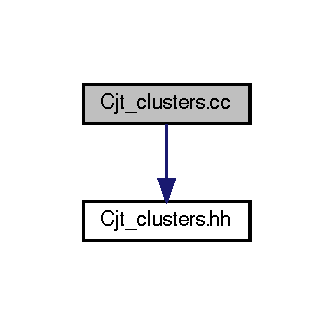
\includegraphics[width=160pt]{_cjt__clusters_8cc__incl}
\end{center}
\end{figure}
\subsection*{Funcions}
\begin{DoxyCompactItemize}
\item 
void \hyperlink{_cjt__clusters_8cc_ac7539e7b223cc6042be093b32ac8b016}{imprimir\+\_\+arbre} (const Bin\+Tree$<$ pair$<$ string, double $>$$>$ \&arbre)
\begin{DoxyCompactList}\small\item\em Imprimeix un arbre. \end{DoxyCompactList}\end{DoxyCompactItemize}


\subsection{Descripció Detallada}
Implementació de la classe \hyperlink{class_cjt__clusters}{Cjt\+\_\+clusters}. 



\subsection{Documentació de les Funcions}
\mbox{\Hypertarget{_cjt__clusters_8cc_ac7539e7b223cc6042be093b32ac8b016}\label{_cjt__clusters_8cc_ac7539e7b223cc6042be093b32ac8b016}} 
\index{Cjt\+\_\+clusters.\+cc@{Cjt\+\_\+clusters.\+cc}!imprimir\+\_\+arbre@{imprimir\+\_\+arbre}}
\index{imprimir\+\_\+arbre@{imprimir\+\_\+arbre}!Cjt\+\_\+clusters.\+cc@{Cjt\+\_\+clusters.\+cc}}
\subsubsection{\texorpdfstring{imprimir\+\_\+arbre()}{imprimir\_arbre()}}
{\footnotesize\ttfamily void imprimir\+\_\+arbre (\begin{DoxyParamCaption}\item[{const Bin\+Tree$<$ pair$<$ string, double $>$$>$ \&}]{arbre }\end{DoxyParamCaption})}



Imprimeix un arbre. 

\begin{DoxyPrecond}{Precondició}
El double de les fulles és igual a -\/1 
\end{DoxyPrecond}
\begin{DoxyPostcond}{Postcondició}
S\textquotesingle{}ha imprès l\textquotesingle{}arbre pel canal estàndard de sortida 
\end{DoxyPostcond}


Definició a la línia 9 del fitxer Cjt\+\_\+clusters.\+cc.


\begin{DoxyCode}
9                                                               \{
10     \textcolor{keywordflow}{if}(arbre.value().second == -1) cout << \textcolor{stringliteral}{"["} << arbre.value().first << \textcolor{stringliteral}{"]"};
11     \textcolor{keywordflow}{else}\{
12         cout << \textcolor{stringliteral}{"[("} << arbre.value().first << \textcolor{stringliteral}{", "} << arbre.value().second << \textcolor{stringliteral}{") "};
13         \hyperlink{_cjt__clusters_8cc_ac7539e7b223cc6042be093b32ac8b016}{imprimir\_arbre}(arbre.left());
14         \hyperlink{_cjt__clusters_8cc_ac7539e7b223cc6042be093b32ac8b016}{imprimir\_arbre}(arbre.right());
15         cout << \textcolor{stringliteral}{"]"};
16     \}
17 \}
\end{DoxyCode}

\hypertarget{_cjt__clusters_8hh}{}\section{Referència del Fitxer Cjt\+\_\+clusters.\+hh}
\label{_cjt__clusters_8hh}\index{Cjt\+\_\+clusters.\+hh@{Cjt\+\_\+clusters.\+hh}}


Especificació de la classe \hyperlink{class_cjt__clusters}{Cjt\+\_\+clusters}.  


\subsection*{Classes}
\begin{DoxyCompactItemize}
\item 
class \hyperlink{class_cjt__clusters}{Cjt\+\_\+clusters}
\begin{DoxyCompactList}\small\item\em Representa el conjunt de clusters i les operacions que aquests permeten. \end{DoxyCompactList}\end{DoxyCompactItemize}


\subsection{Descripció Detallada}
Especificació de la classe \hyperlink{class_cjt__clusters}{Cjt\+\_\+clusters}. 


\hypertarget{_cjt__especies_8cc}{}\section{Referència del Fitxer Cjt\+\_\+especies.\+cc}
\label{_cjt__especies_8cc}\index{Cjt\+\_\+especies.\+cc@{Cjt\+\_\+especies.\+cc}}


Implementació de la classe \hyperlink{_cjt__especies_8cc}{Cjt\+\_\+especies.\+cc}.  


Inclou el graf de dependències per a Cjt\+\_\+especies.\+cc\+:
\nopagebreak
\begin{figure}[H]
\begin{center}
\leavevmode
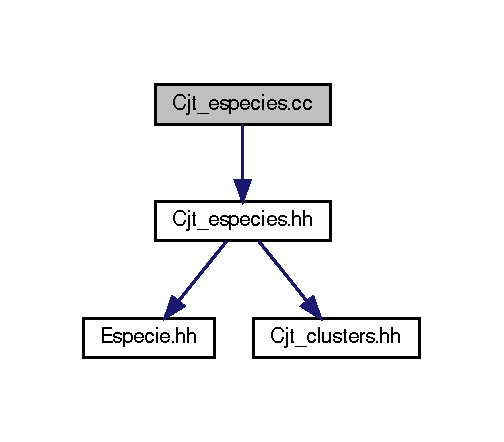
\includegraphics[width=242pt]{_cjt__especies_8cc__incl}
\end{center}
\end{figure}


\subsection{Descripció Detallada}
Implementació de la classe \hyperlink{_cjt__especies_8cc}{Cjt\+\_\+especies.\+cc}. 


\hypertarget{_cjt__especies_8hh}{}\section{Referència del Fitxer Cjt\+\_\+especies.\+hh}
\label{_cjt__especies_8hh}\index{Cjt\+\_\+especies.\+hh@{Cjt\+\_\+especies.\+hh}}


Especificació de la classe \hyperlink{class_cjt__especies}{Cjt\+\_\+especies}.  


Inclou el graf de dependències per a Cjt\+\_\+especies.\+hh\+:
\nopagebreak
\begin{figure}[H]
\begin{center}
\leavevmode
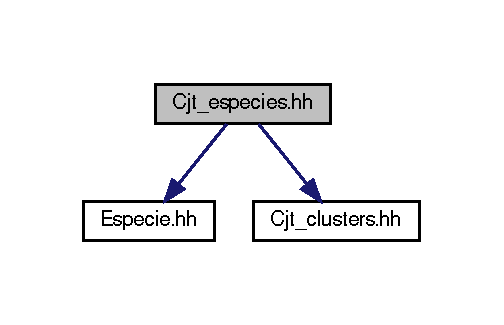
\includegraphics[width=242pt]{_cjt__especies_8hh__incl}
\end{center}
\end{figure}
\subsection*{Classes}
\begin{DoxyCompactItemize}
\item 
class \hyperlink{class_cjt__especies}{Cjt\+\_\+especies}
\begin{DoxyCompactList}\small\item\em Representa el conjunt d\textquotesingle{}espècies i les operacions que permet. \end{DoxyCompactList}\end{DoxyCompactItemize}


\subsection{Descripció Detallada}
Especificació de la classe \hyperlink{class_cjt__especies}{Cjt\+\_\+especies}. 


\hypertarget{_especie_8cc}{}\section{Referència del Fitxer Especie.\+cc}
\label{_especie_8cc}\index{Especie.\+cc@{Especie.\+cc}}


Implementació de la classe \hyperlink{class_especie}{Especie}.  


Inclou el graf de dependències per a Especie.\+cc\+:\nopagebreak
\begin{figure}[H]
\begin{center}
\leavevmode
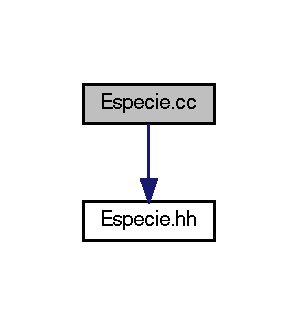
\includegraphics[width=143pt]{_especie_8cc__incl}
\end{center}
\end{figure}


\subsection{Descripció Detallada}
Implementació de la classe \hyperlink{class_especie}{Especie}. 


\hypertarget{_especie_8hh}{}\section{Referència del Fitxer Especie.\+hh}
\label{_especie_8hh}\index{Especie.\+hh@{Especie.\+hh}}


Especificació de la classe \hyperlink{class_especie}{Especie}.  


\subsection*{Classes}
\begin{DoxyCompactItemize}
\item 
class \hyperlink{class_especie}{Especie}
\begin{DoxyCompactList}\small\item\em Representa una espècie amb els seus atributs i les seves operacions. \end{DoxyCompactList}\end{DoxyCompactItemize}


\subsection{Descripció Detallada}
Especificació de la classe \hyperlink{class_especie}{Especie}. 


\hypertarget{program_8cc}{}\section{Referència del Fitxer program.\+cc}
\label{program_8cc}\index{program.\+cc@{program.\+cc}}


Programa que conté el main que consisteix en donar diferents operacions.  


Inclou el graf de dependències per a program.\+cc\+:
\nopagebreak
\begin{figure}[H]
\begin{center}
\leavevmode
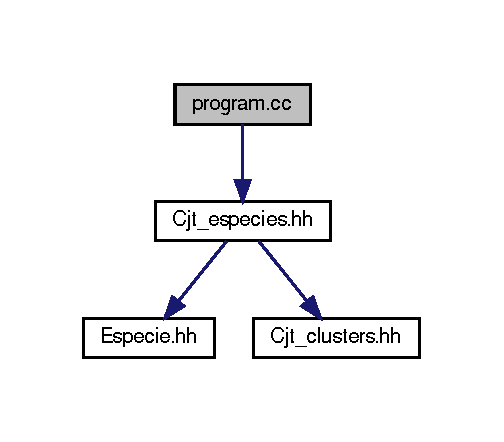
\includegraphics[width=242pt]{program_8cc__incl}
\end{center}
\end{figure}
\subsection*{Funcions}
\begin{DoxyCompactItemize}
\item 
int \hyperlink{program_8cc_ae66f6b31b5ad750f1fe042a706a4e3d4}{main} ()
\begin{DoxyCompactList}\small\item\em Main amb totes les operacions que requereix la pràctica. \end{DoxyCompactList}\end{DoxyCompactItemize}


\subsection{Descripció Detallada}
Programa que conté el main que consisteix en donar diferents operacions. 



\subsection{Documentació de les Funcions}
\mbox{\Hypertarget{program_8cc_ae66f6b31b5ad750f1fe042a706a4e3d4}\label{program_8cc_ae66f6b31b5ad750f1fe042a706a4e3d4}} 
\index{program.\+cc@{program.\+cc}!main@{main}}
\index{main@{main}!program.\+cc@{program.\+cc}}
\subsubsection{\texorpdfstring{main()}{main()}}
{\footnotesize\ttfamily int main (\begin{DoxyParamCaption}{ }\end{DoxyParamCaption})}



Main amb totes les operacions que requereix la pràctica. 



Definició a la línia 53 del fitxer program.\+cc.


\begin{DoxyCode}
53           \{
54     \textcolor{keywordtype}{int} k;
55     cin >> k;
56     \hyperlink{class_especie_a30e274da0f6d1ee4c450702a3f914ecf}{Especie::definir\_k}(k);
57 
58     \hyperlink{class_cjt__especies}{Cjt\_especies} especies;
59     \hyperlink{class_cjt__clusters}{Cjt\_clusters} clusters;
60 
61     \textcolor{keywordtype}{string} op;
62 
63     \textcolor{keywordflow}{while}(cin >> op and op != \textcolor{stringliteral}{"fin"})\{
64         \textcolor{keywordtype}{string} gen, id;
65 
66         \textcolor{keywordflow}{if}(op == \textcolor{stringliteral}{"crea\_especie"})\{
67             cin >> \textcolor{keywordtype}{id} >> gen;
68             cout << \textcolor{stringliteral}{"# "} << op << \textcolor{stringliteral}{" "} << \textcolor{keywordtype}{id} << \textcolor{stringliteral}{" "} << gen << endl;
69             \textcolor{keywordflow}{if}(not especies.\hyperlink{class_cjt__especies_a7fa2f303eb4e3065d87174a1c3e71942}{existeix\_especie}(\textcolor{keywordtype}{id})) especies.
      \hyperlink{class_cjt__especies_a542ea997b387b5bac131ba7bcb23aec3}{afegeix\_especie}(\textcolor{keywordtype}{id},gen);
70             \textcolor{keywordflow}{else} cout << \textcolor{stringliteral}{"ERROR: La especie "} << \textcolor{keywordtype}{id} << \textcolor{stringliteral}{" ya existe."} << endl;
71             cout << endl;
72         \}
73         \textcolor{keywordflow}{else} \textcolor{keywordflow}{if}(op == \textcolor{stringliteral}{"obtener\_gen"})\{
74             cin >> id;
75             cout << \textcolor{stringliteral}{"# "} << op << \textcolor{stringliteral}{" "} << \textcolor{keywordtype}{id} << endl;
76             \textcolor{keywordflow}{if}(especies.\hyperlink{class_cjt__especies_a7fa2f303eb4e3065d87174a1c3e71942}{existeix\_especie}(\textcolor{keywordtype}{id})) cout << especies.
      \hyperlink{class_cjt__especies_ae6c9a86512b2ed7686741459167b68c9}{obtenir\_gen}(\textcolor{keywordtype}{id}) << endl;
77             \textcolor{keywordflow}{else} cout << \textcolor{stringliteral}{"ERROR: La especie "} << \textcolor{keywordtype}{id} << \textcolor{stringliteral}{" no existe."} << endl;
78             cout << endl;
79         \}
80         \textcolor{keywordflow}{else} \textcolor{keywordflow}{if}(op == \textcolor{stringliteral}{"distancia"})\{
81             \textcolor{keywordtype}{string} id2;
82             cin >> \textcolor{keywordtype}{id} >> id2;
83             cout << \textcolor{stringliteral}{"# "} << op << \textcolor{stringliteral}{" "} << \textcolor{keywordtype}{id} << \textcolor{stringliteral}{" "} << id2 << endl;
84             \textcolor{keywordflow}{if}(especies.\hyperlink{class_cjt__especies_a7fa2f303eb4e3065d87174a1c3e71942}{existeix\_especie}(\textcolor{keywordtype}{id}) and especies.
      \hyperlink{class_cjt__especies_a7fa2f303eb4e3065d87174a1c3e71942}{existeix\_especie}(id2))\{
85                 cout << especies.\hyperlink{class_cjt__especies_abcea459e5b302c0eda1583b1dc571bff}{consultar\_distancia}(\textcolor{keywordtype}{id},id2) << endl;
86             \}
87             \textcolor{keywordflow}{else}\{
88                 cout << \textcolor{stringliteral}{"ERROR: La especie "};
89                 \textcolor{keywordflow}{if}(especies.\hyperlink{class_cjt__especies_a7fa2f303eb4e3065d87174a1c3e71942}{existeix\_especie}(\textcolor{keywordtype}{id})) cout << id2 << \textcolor{stringliteral}{" no existe."};
90                 \textcolor{keywordflow}{else} \textcolor{keywordflow}{if}(especies.\hyperlink{class_cjt__especies_a7fa2f303eb4e3065d87174a1c3e71942}{existeix\_especie}(id2)) cout << \textcolor{keywordtype}{id} << \textcolor{stringliteral}{" no existe."};
91                 \textcolor{keywordflow}{else} cout << \textcolor{keywordtype}{id} << \textcolor{stringliteral}{" y la especie "} << id2 << \textcolor{stringliteral}{" no existen."};
92                 cout << endl;
93             \}
94             cout << endl;
95         \}
96         \textcolor{keywordflow}{else} \textcolor{keywordflow}{if}(op == \textcolor{stringliteral}{"elimina\_especie"})\{
97             cin >> id;
98             cout << \textcolor{stringliteral}{"# "} << op << \textcolor{stringliteral}{" "} << \textcolor{keywordtype}{id} << endl;
99             \textcolor{keywordflow}{if}(especies.\hyperlink{class_cjt__especies_a7fa2f303eb4e3065d87174a1c3e71942}{existeix\_especie}(\textcolor{keywordtype}{id})) especies.
      \hyperlink{class_cjt__especies_a6de3583aff6835d743fc9493c7b38576}{eliminar\_especie}(\textcolor{keywordtype}{id});
100             \textcolor{keywordflow}{else} cout << \textcolor{stringliteral}{"ERROR: La especie "} << \textcolor{keywordtype}{id} << \textcolor{stringliteral}{" no existe."} << endl;
101             cout << endl;
102         \}
103         \textcolor{keywordflow}{else} \textcolor{keywordflow}{if}(op == \textcolor{stringliteral}{"existe\_especie"})\{
104             cin >> id;
105             cout << \textcolor{stringliteral}{"# "} << op << \textcolor{stringliteral}{" "} << \textcolor{keywordtype}{id} << endl;
106             \textcolor{keywordflow}{if}(especies.\hyperlink{class_cjt__especies_a7fa2f303eb4e3065d87174a1c3e71942}{existeix\_especie}(\textcolor{keywordtype}{id})) cout << \textcolor{stringliteral}{"SI"} << endl;
107             \textcolor{keywordflow}{else} cout << \textcolor{stringliteral}{"NO"} << endl;
108             cout << endl;
109         \}
110         \textcolor{keywordflow}{else} \textcolor{keywordflow}{if}(op == \textcolor{stringliteral}{"lee\_cjt\_especies"})\{
111             cout << \textcolor{stringliteral}{"# "} << op << endl << endl;
112             especies.\hyperlink{class_cjt__especies_a12bd759f16126d0e34b06ecf15575456}{llegir\_cjt\_especies}();
113         \}
114         \textcolor{keywordflow}{else} \textcolor{keywordflow}{if}(op == \textcolor{stringliteral}{"imprime\_cjt\_especies"})\{
115             cout << \textcolor{stringliteral}{"# "} << op << endl;
116             especies.\hyperlink{class_cjt__especies_a8bc985ceafb3bb0e5f3c68ba52a36e86}{escriure\_cjt\_especies}();
117             cout << endl;
118         \}
119         \textcolor{keywordflow}{else} \textcolor{keywordflow}{if}(op == \textcolor{stringliteral}{"tabla\_distancias"})\{
120             cout << \textcolor{stringliteral}{"# "} << op << endl;
121             especies.\hyperlink{class_cjt__especies_aeb2402fbb6b5cc5eeea31981c51110bc}{imprimir\_taula\_distancies}();
122             cout << endl;
123         \}
124         \textcolor{keywordflow}{else} \textcolor{keywordflow}{if}(op == \textcolor{stringliteral}{"inicializa\_clusters"})\{
125             cout << \textcolor{stringliteral}{"# "} << op << endl;
126             especies.\hyperlink{class_cjt__especies_a568357e9132b16cfe7280e29e6e89cfb}{inicialitza\_clusters}(clusters);
127             clusters.\hyperlink{class_cjt__clusters_a2ee45d5dabc656adf8d7d356239f57c6}{imprimir\_taula\_distancies}();
128             cout << endl;
129         \}
130         \textcolor{keywordflow}{else} \textcolor{keywordflow}{if}(op == \textcolor{stringliteral}{"ejecuta\_paso\_wpgma"})\{
131             cout << \textcolor{stringliteral}{"# "} << op << endl;
132             \textcolor{keywordflow}{if}(clusters.\hyperlink{class_cjt__clusters_a6a240452c7964e1d6b7d54df7ee58563}{num\_clusters}() > 1)\{
133                 clusters.\hyperlink{class_cjt__clusters_a0675e6339f6a8fad8219518c377fbcf9}{pas\_wpgma}();
134                 clusters.\hyperlink{class_cjt__clusters_a2ee45d5dabc656adf8d7d356239f57c6}{imprimir\_taula\_distancies}();
135             \}
136             \textcolor{keywordflow}{else} cout << \textcolor{stringliteral}{"ERROR: num\_clusters <= 1"} << endl;
137             cout << endl;
138         \}
139         \textcolor{keywordflow}{else} \textcolor{keywordflow}{if}(op == \textcolor{stringliteral}{"imprime\_arbol\_filogenetico"})\{
140             cout << \textcolor{stringliteral}{"# "} << op << endl;
141             especies.\hyperlink{class_cjt__especies_a568357e9132b16cfe7280e29e6e89cfb}{inicialitza\_clusters}(clusters);
142             \textcolor{keywordflow}{if}(especies.\hyperlink{class_cjt__especies_a2539f8918c40587579e1b98be28bdddc}{consultar\_mida}() > 0)\{
143                 clusters.\hyperlink{class_cjt__clusters_a952291f47c4dd2edf62b3c110bee24f2}{imprimeix\_arbre\_filogenetic}();
144                 cout << endl;
145             \}
146             \textcolor{keywordflow}{else} cout << \textcolor{stringliteral}{"ERROR: El conjunto de clusters es vacio."} << endl;
147             cout << endl;
148         \}
149         \textcolor{keywordflow}{else} \textcolor{keywordflow}{if}(op == \textcolor{stringliteral}{"imprime\_cluster"})\{
150             cin >> id;
151             cout << \textcolor{stringliteral}{"# "} << op << \textcolor{stringliteral}{" "} << \textcolor{keywordtype}{id} << endl;
152             \textcolor{keywordflow}{if}(clusters.\hyperlink{class_cjt__clusters_af85ce29152ee18987f391a2d27af59b5}{existeix\_cluster}(\textcolor{keywordtype}{id}))\{
153                 clusters.\hyperlink{class_cjt__clusters_a732366a2fd16153e162fd838d25b5a56}{imprimeix\_cluster}(\textcolor{keywordtype}{id});
154                 cout << endl;
155             \}
156             \textcolor{keywordflow}{else} cout << \textcolor{stringliteral}{"ERROR: El cluster "} << \textcolor{keywordtype}{id} << \textcolor{stringliteral}{" no existe."} << endl;
157             cout << endl;
158         \}
159     \}
160 \}
\end{DoxyCode}

%--- End generated contents ---

% Index
\backmatter
\newpage
\phantomsection
\clearemptydoublepage
\addcontentsline{toc}{chapter}{Índex}
\printindex

\end{document}
